%----------------------------------------------------------------------------------------
% Bachelorarbeit IGS
% Report LaTeX template (English)
% Interactive Graphics and Simulation Group
% University of Innsbruck
%----------------------------------------------------------------------------------------

\documentclass[11pt,a4paper,twoside,openright]{report}

%----------------------------------------------------------------------------------------
% Include required packages
\usepackage{graphicx}
\graphicspath{ {./images/} }
\usepackage{amsmath}
\usepackage{amssymb}
\usepackage{listings}
\usepackage{color}
\usepackage{adjustbox}
\usepackage{makecell}
\usepackage{pgfplots}

\definecolor{codegreen}{rgb}{0,0.6,0}
\definecolor{codegray}{rgb}{0.5,0.5,0.5}
\definecolor{codepurple}{rgb}{0.58,0,0.82}
\definecolor{backcolour}{rgb}{0.95,0.95,0.92}

\lstdefinestyle{mystyle}{
    backgroundcolor=\color{backcolour},
    commentstyle=\color{codegreen},
    keywordstyle=\color{magenta},
    numberstyle=\tiny\color{codegray},
    stringstyle=\color{codepurple},
    basicstyle=\footnotesize,
    breakatwhitespace=false,
    breaklines=true,
    captionpos=b,
    keepspaces=true,
    numbers=left,
    numbersep=5pt,
    showspaces=false,
    showstringspaces=false,
    showtabs=false,
    tabsize=2
}

\lstset{style=mystyle}
\usepackage{cleveref}

\usepackage[english]{babel}
%\usepackage[ngerman]{babel}

\usepackage[utf8x]{inputenc}
\usepackage[T1]{fontenc}

\usepackage{fancyhdr}
\usepackage{emptypage}

\usepackage[left=2.7cm, right=2.7cm, top=3cm]{geometry}

%----------------------------------------------------------------------------------------
% Start document

\begin{document}


%----------------------------------------------------------------------------------------
% Title page
%----------------------------------------------------------------------------------------

\begin{titlepage} % User-defined title page

\begin{center}

\includegraphics[width=1.2cm]{images/uibk}

\begin{large}
Leopold-Franzens-Universität Innsbruck\\[5mm]
Institute of Computer Science\\
Interactive Graphics and Simulation Group\\[25mm]
\end{large}

Bachelor Thesis\\[15mm]

{\LARGE \bf Procedural Generation of Mountain Ranges Based on Geology}\\[15mm]

Bernhard Fritz\\
\texttt{bernhard.e.fritz@student.uibk.ac.at}\\[35mm]

advised by\\
Univ.-Prof. Dipl.-Inf. Matthias Harders\\[10mm]

\vfill

Innsbruck, \today
\end{center}

\end{titlepage}

\pagenumbering{roman}




%----------------------------------------------------------------------------------------
% Abstract
%----------------------------------------------------------------------------------------
\chapter*{Abstract}
In this thesis several geological phenomena were inspected in terms of what impact they have on landscape and how they can be implemented algorithmically.
\medskip
\noindent \\\textbf{Keywords} keyword1, keyword2.


%----------------------------------------------------------------------------------------
% Tables and lists of document material
%----------------------------------------------------------------------------------------

\tableofcontents
\listoffigures
\listoftables


%----------------------------------------------------------------------------------------
% Declaration
%----------------------------------------------------------------------------------------
\chapter*{Declaration}
By my own signature I declare that I produced this work as the sole author, working independently,
and that I did not use any sources and aids other than those referenced in the text.
All passages borrowed from external sources, verbatim or by content, are explicitly identified as
such.\\

\vspace{15mm}

\noindent Signature: \underline{\hspace{5cm}} \hspace{1cm}  Date: \underline{\hspace{5cm}}


%----------------------------------------------------------------------------------------
% Main body
%----------------------------------------------------------------------------------------
\chapter{Introduction}
\label{sec:intro}

\pagenumbering{arabic}
\pagestyle{fancy}

Being born in Tyrol, a mountainous area of Austria, made me curious about how mountains like these surrounding my homeland came into existance in the first place. According to my research, there still is no scientific consensus on what geological processes were involved in the creation of these rock formations originally. My interest in computer graphics allowed me to grasp geological phenomena like tectonic plate movement as well as various types of erosion hands-on in terms of implementing algorithms and simulations that imitate said behaviour.

The foundation of all algorithms and simulations discussed in this bachelor thesis are heightmaps and heightmap transformations. A heightmap is a concept in computer graphics that allows to model landscapes in an efficient way, meaning that their height is well-defined for any coordinate tuple $(x,z)$. Due to this, it is possible to export heightmaps as grayscale image files. This process is described in detail in \cref{subsec:exportingheightmaps}. Heightmaps consist of a predefined number of tiles. These tiles again consist of 2 triangles each as depicted in \cref{fig:heightmapgrid}.

\begin{figure}[h]
\centering
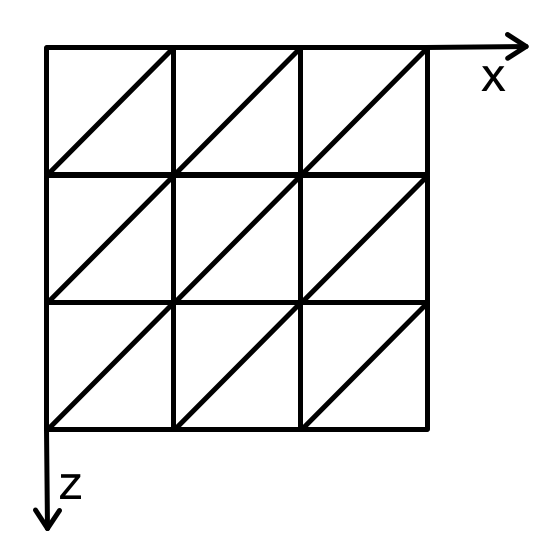
\includegraphics[width=0.25\linewidth]{heightmapgrid.png}
\caption{Heightmap grid}\label{fig:heightmapgrid}
\end{figure}

When speaking of heightmap resolution one can refer to the number of tiles it consists of. Usually heightmaps have square dimensions, meaning the number of columns and rows of tiles is the same.

To model the geological phenomena responsible for the creation of mountain ranges found on earth, it is necessary to have a basic understanding of how they work. As research suggests, tectonic plate movement is one of the main contributors when it comes to generation of rock formations. The key principles of plate tectonics are based on the two essential layers earth consists of, the lithosphere and asthenosphere. The cool and rigid lithosphere is divided in distinct tectonic plates which float on top of the hot, fluid-like asthenosphere. There are several ways lithospheric plates can interact with each other:
\begin{itemize}
  \item They can grind past each other which results in strong earthquakes leaving the plates involved in this process essentially unaffected.
  \item They can slide apart from each other which results in volcanic activity along the  boundaries of the plates involved.
  \item They can slide toward each other and cause one plate to move underneath the other or they can collide and pile up.
\end{itemize}
\Cref{sec:tectonicplatesimulation} contains more information about how these geological processes were implemented algorithmically.
Tectonic plate movement is only one of many geological phenomena that directly influences shape and appearance of mountain ranges. Mountain features like distinct summits, ravines, valleys and cliffs are product of another type of geological phenomenon called erosion.

Erosion describes the processes involved in the transportation of soil, rock or dissolved material from one location to another. The driving forces responsible for this phenomenon are:
\begin{itemize}
  \item Water (i.e. hydraulic erosion)
  \item Wind (i.e. wind erosion)
  \item Ice (i.e. glacial erosion)
  \item Gravity (i.e. thermal erosion)
\end{itemize}


%----------------------------------------------------------------------------------------
\chapter{Related Work}
\label{sec:related}
Kamal and Uddin evaluated various terrain generation algorithms like Diamond-Square-Algorithm and Fault-Algorithm and came up with their own algorithm called Repeated Magnification and Probing \cite{Kamal:2007:PCT:1321261.1321264}. Thermal and hydraulic erosion algorithms were first described by Musgrave \cite{Musgrave:1989:SRE:74333.74337}. Based on Musgraves work, Olsen implemented his own version of thermal and hydraulic erosion algorithm and also improved them performance-wise to make them available for realtime-applications \cite{Olsen:2004}. Vitanen describes the theoretical foundation of plate tectonics, compares several existing applications and ultimately implements his own tectonic plate simulation \cite{Vitanen:2012}.
%----------------------------------------------------------------------------------------
\chapter{Methods}
\label{sec:methods}

\section{Diamond-Square algorithm}
This algorithm was first introduced by Fournier et al in 1982 \cite{Fournier:1982:CRS:358523.358553}. It can be considered as an extension of Midpoint-Displacement (MPD) algorithm. By recursively subdividing a line into segments of equal length and displacing the resulting midpoints by a random amount, MPD algorithm is able to produce a fairly arbitrary looking 1D-landscape. \Cref{fig:mpd0,fig:mpd1,fig:mpd2} depict the first 2 iterations of MPD algorithm.

\begin{figure}[!htb]
\minipage{0.33\textwidth}
  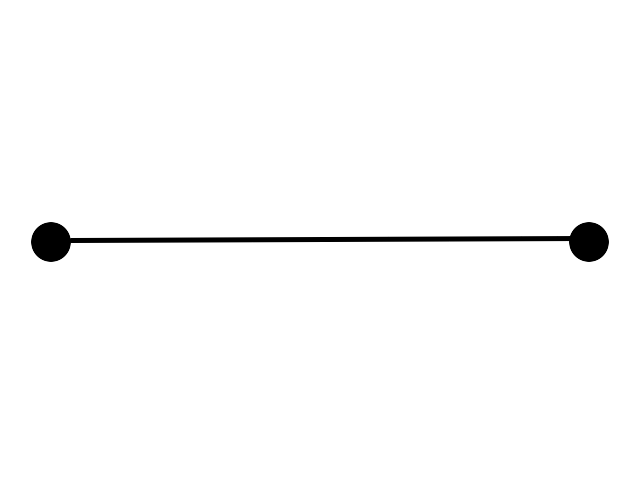
\includegraphics[width=\linewidth]{mpd0.png}
  \caption{MPD initialization}\label{fig:mpd0}
\endminipage\hfill
\minipage{0.33\textwidth}
  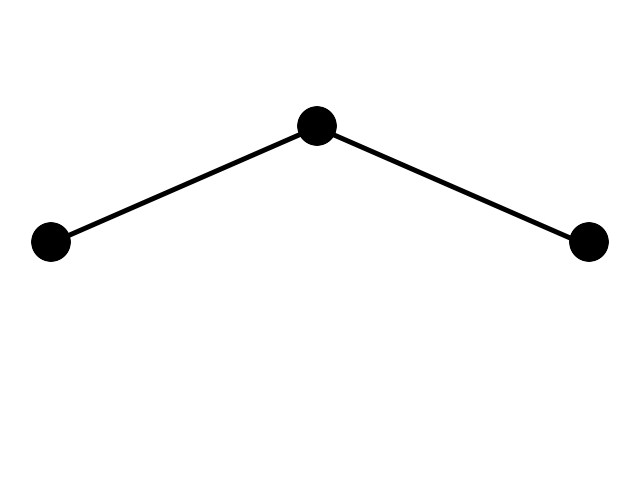
\includegraphics[width=\linewidth]{mpd1.png}
  \caption{MPD iteration 1}\label{fig:mpd1}
\endminipage\hfill
\minipage{0.33\textwidth}%
  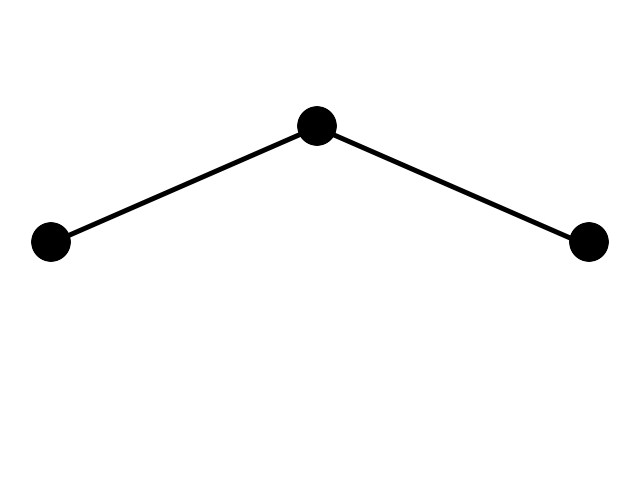
\includegraphics[width=\linewidth]{mpd2.png}
  \caption{MPD iteration 2}\label{fig:mpd2}
\endminipage
\end{figure}

\noindent To take MPD algorithm to the next level Diamond-Square algorithm allows to procedurally generate 2D-landscape. During initialization, Diamond-Square algorithm raises the heightmap's corner vertices to an arbitrary height. Once the corner vertices have been initialized a \emph{Diamond-Step} followed by a \emph{Square-Step} will be performed in an alternating fashion until all vertices have been initialized. The following pseudocode will demonstrate how Diamond-Square algorithm can be implemented:

\begin{lstlisting}[caption=DS pseudocode, mathescape=true]
function randomFloat(range):
  return a random floating point number $\in$ [0, range)

procedure diamondStep(hm, roughness, left, right, top, bottom):
  midpointColumn = left+(right-left)/2
  midpointRow = top+(bottom-top)/2
  avgHeight = ... // average height of square corners
  r = roughness * (randomFloat(2)-1)
  hm.setHeightAt(midpointColumn, midpointRow, avgHeight+r)

procedure squareStep(hm, roughness, left, right, top, bottom):
  midpointColumn = left+(right-left)/2
  midpointRow = top+(bottom-top)/2
  avgHeightTop = ... // average height of top diamond corners
  r = roughness * (randomFloat(2)-1)
  hm.setHeightAt(midpointColumn, top, avgHeightTop+r)
  ... // similar steps for left, right and bottom diamond

procedure ds(hm, roughness, left, right, top, bottom):
  diamondStep(hm, roughness, left, right, top, bottom)
  squareStep(hm, roughtness, left, right, top, bottom)

procedure perform(hm, roughness):
  columns = hm.getColumns()
  rows = hm.getRows()

  // initialize heightmap corners
  hm.setHeightAt(0, 0, roughness)
  hm.setHeightAt(columns, 0, roughness)
  hm.setHeightAt(0, rows, roughness)
  hm.setHeightAt(columns, rows, roughness)

  while columns > 1:
    for row = 0; row < hm.getRows(); row += rows:
      for column = 0; column < hm.getColumns(); column += columns:
        ds(hm, roughness, column, column+columns, row, row+rows)
    roughness /= 2.0
    columns /= 2
    rows /= 2
\end{lstlisting}

\noindent \Cref{fig:ds1,fig:ds2,fig:ds3,fig:ds4,fig:ds5} depict the Diamond-Square algorithm applied to a 4x4 heightmap. Orange vertices are being altered in height, while blue vertices contribute to the average height calculation.

\begin{figure}[!htb]
\minipage{0.33\textwidth}
  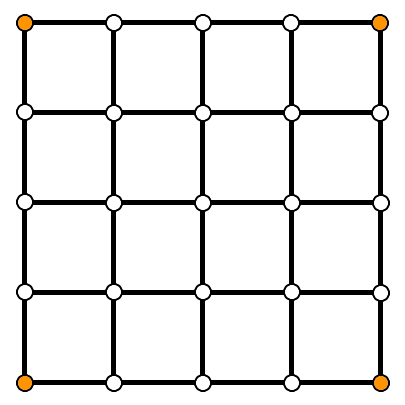
\includegraphics[width=\linewidth]{ds1.png}
  \caption{Diamond-Square initialization}\label{fig:ds1}
\endminipage
\minipage{0.33\textwidth}
  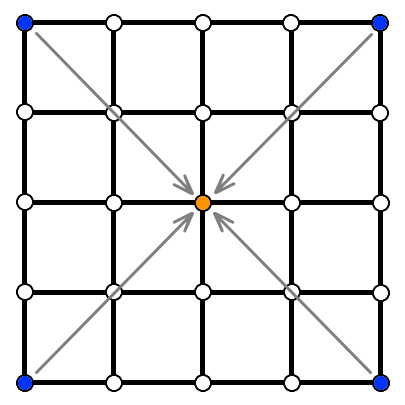
\includegraphics[width=\linewidth]{ds2.png}
  \caption{Diamond-Step 1}\label{fig:ds2}
\endminipage
\minipage{0.33\textwidth}%
  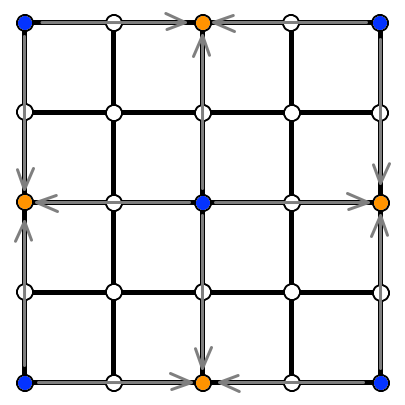
\includegraphics[width=\linewidth]{ds3.png}
  \caption{Square-Step 1}\label{fig:ds3}
\endminipage\hfill
\\
\centering
\minipage{0.33\textwidth}
  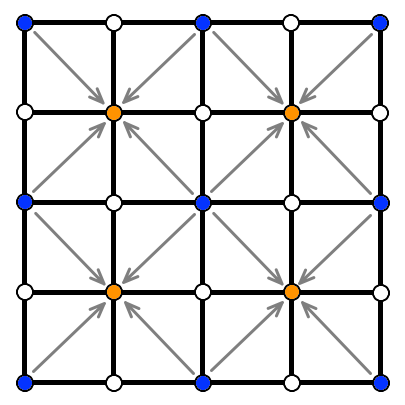
\includegraphics[width=\linewidth]{ds4.png}
  \caption{Diamond-Step 2}\label{fig:ds4}
\endminipage
\minipage{0.33\textwidth}%
  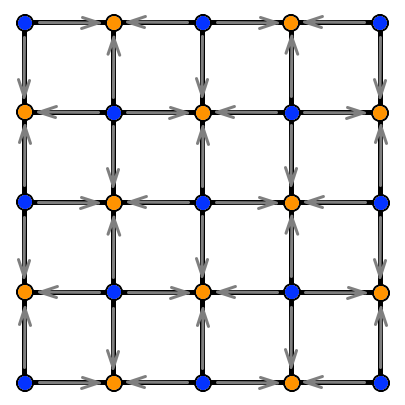
\includegraphics[width=\linewidth]{ds5.png}
  \caption{Square-Step 2}\label{fig:ds5}
\endminipage
\end{figure}

\section{Fault algorithm}
This algorithm was first described by Krten \cite{Krten:1994}. He proposed to randomly draw a line across the heightmap and split the landscape into two regions. By raising one and lowering the other region and repeating the whole process several times, interesting mountain-like features can emerge. Due to the sheer randomness of this algorithm it is impossible to control the position, shape or spread of the resulting mountains. However, it is possible to control the roughness of the generated terrain by adjusting the amount by which vertices get raised or lowered per iteration.

To determine if a heightmap vertex needs to be raised or lowered, a boolean function called \emph{raise} will be used. Function \emph{raise} is defined as follows:
\begin{align*}
sgn(x) &=
\begin{cases}
  -1 & \text{if}\ x < 0, \\
  0 & \text{if}\ x = 0, \\
  1 & \text{if}\ x > 0.
\end{cases} \\
\mathbf{v} &= (v_1\ v_2\ v_3)^\intercal \\
raise(\mathbf{v}) &=
\begin{cases}
  0 & \text{if}\ sgn(v_2) = -1, \\
  1 & \text{if}\ sgn(v_2) \geq 0.
\end{cases}
\end{align*}
Let vectors $\mathbf{a}$ and $\mathbf{b}$ describe a random cutting line. Then a vertex pointed to by vector $\mathbf{p}$ will be raised in height if $raise((\mathbf{p}-\mathbf{a}) \times (\mathbf{b} - \mathbf{a}))$ equals 1 and lowered otherwise. \Cref{fig:fault0,fig:fault1,fig:fault2,fig:fault3} will depict the first 3 iterations of Fault algorithm using different shades of green. Light green represents high and dark green low elevation respectively.

\begin{figure}[!htb]
\minipage{0.24\textwidth}
  
\includegraphics[width=\linewidth]{fault0.png}
  \caption{Fault initialization}\label{fig:fault0}
\endminipage\hfill
\minipage{0.24\textwidth}
  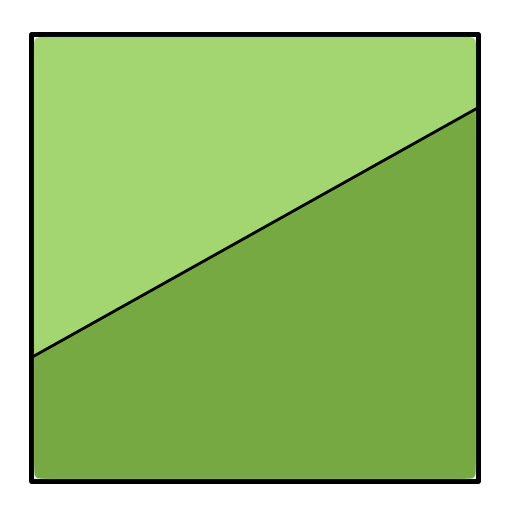
\includegraphics[width=\linewidth]{fault2.png}
  \caption{Fault iteration 1}\label{fig:fault1}
\endminipage\hfill
\minipage{0.24\textwidth}
  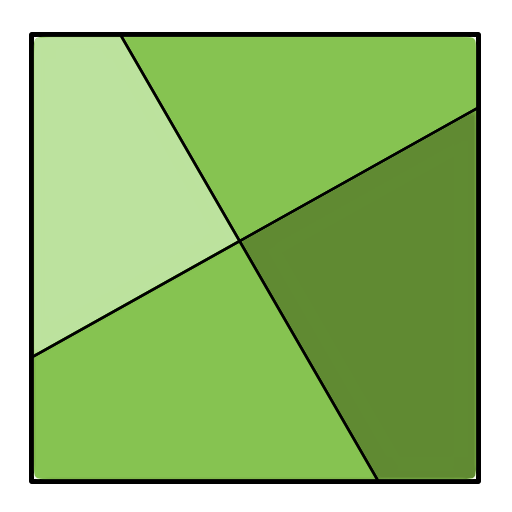
\includegraphics[width=\linewidth]{fault4.png}
  \caption{Fault iteration 2}\label{fig:fault2}
\endminipage\hfill
\minipage{0.24\textwidth}%
  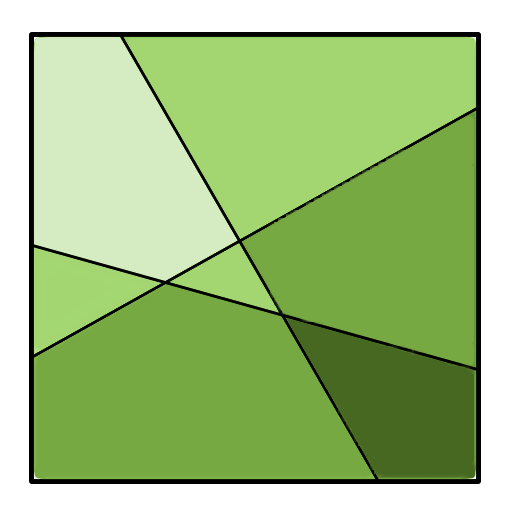
\includegraphics[width=\linewidth]{fault6.png}
  \caption{Fault iteration 3}\label{fig:fault3}
\endminipage
\end{figure}

\section{RMP algorithm}
RMP stands for \emph{Repeated Magnification and Probing}, was created by Kamal and Uddin \cite{Kamal:2007:PCT:1321261.1321264} and can be categorized as parametrically controllable mountain generation algorithm. Height, spread and location of the mountain can be controlled by parameters. This algorithm is similar to Fault algorithm, meaning that only selected regions are repeatedly altered in height. The process how these regions are obtained is not described in Kamal and Uddin's paper \cite{Kamal:2007:PCT:1321261.1321264}. In \cref{subsec:graphbasedimpl,subsec:voronoibasedimpl} two techniques will be presented that are capable of generating randomly distributed polygon-like shapes which can be used for RMP algorithm.

\subsection{Graph-based implementation}
\label{subsec:graphbasedimpl}
This implementation starts by placing 4 lines along the landscape borders as well as $l$ randomly distributed cutting lines all over the landscape. In the next step all line intersections will be determined. To determine if two lines intersect i.e. they share a point that lies on both lines, following equation system has to be solved:
\begin{align}
\mathbf{p} &= \mathbf{a} + u * \mathbf{d} \label{eq:rayrayint1}\\
\mathbf{p} &= \mathbf{b} + v * \mathbf{e} \label{eq:rayrayint2}
\intertext{The following notation is used to the extract a vector's x- and y-coordinates:}
\mathbf{v} &= (v_1\ v_2)^\intercal \label{eq:rayrayint3}
\intertext{Expanding \cref{eq:rayrayint1,eq:rayrayint2} using notation from \cref{eq:rayrayint3} results in:}
p_1 &= a_1 + u * d_1 \label{eq:rayrayint4}\\
p_2 &= a_2 + u * d_2 \label{eq:rayrayint5}\\
p_1 &= b_1 + v * e_1 \label{eq:rayrayint6}\\
p_2 &= b_2 + v * e_2 \label{eq:rayrayint7}
\intertext{Eliminating $p_1$ and $p_2$ from \cref{eq:rayrayint4,eq:rayrayint5,eq:rayrayint6,eq:rayrayint7} results in:}
a_1 + u * d_1 &= b_1 + v * e_1 \label{eq:rayrayint8}\\
a_2 + u * d_2 &= b_2 + v * e_2 \label{eq:rayrayint9}
\intertext{Solving \cref{eq:rayrayint8} for $u$ results in:}
u &= \frac{b_1 + v * e_1 - a_1}{d_1} \label{eq:rayrayint10}\\
\intertext{Substituting $u$ in \cref{eq:rayrayint9} by \cref{eq:rayrayint10} and solving for $v$ results in:}
v &= \frac{(b_2 - a_2) * d_1 - (b_1 - a_1) * d_2}{e_1 * d_2 - e_2 * d_1} \label{eq:rayrayint11}
\intertext{Substituting $v$ in \cref{eq:rayrayint2} by \cref{eq:rayrayint11} results in $\mathbf{p}$ if the two lines intersect, i.e. they are not parallel.}
\end{align}
These intersections are represented as vertices in an undirected graph. A line can have several intersections. Therefore they will be iterated through from the start of the line to the end. Let $\mathbf{i}$ and $\mathbf{j}$ be two intersections on a line defined by origin $\mathbf{a}$ and direction $\mathbf{d}$ as seen in \cref{eq:rayrayint1}. To determine which intersection is closer to the start of the line one has to substitute $\mathbf{p}$ in \cref{eq:rayrayint1} with $\mathbf{i}$ and $\mathbf{j}$ and solve both resulting equations for $u$. The smaller $u$ gets, the closer it is to the origin of the line. Intersections (i.e. vertices) along a line will be connected in order (closest to farthest) using graph edges. Once the graph is set up, a Depth-First-Search (DFS) based algorithm will be used to determine all minimal cycles. These cycles represent the polygon shapes produced by the previously placed cutting lines. Once the polygons are obtained another undirected graph will be created. This time the vertices of the graph will represent the polygons. In this graph 2 vertices are connected by an edge only if both polygons are next to each other. Once this newly generated graph is set up another DFS will be performed. As start point of this search the polygon which should contain the desired mountain peak is chosen. The combined region of the first $r$ elements of the DFS will be raised in height. A point-in-polygon test, originated by Shirmat \cite{Shimrat:1962:APP:368637.368653} and later implemented in C by W. Randolph Franklin, was used to determine if a heightmap point should be affected by height alterations or not. The whole procedure will be repeated $n$ times. After several tests, it was clear that the graph-based implementation was far too slow to be used for realtime applications. Therefore an alternative implementation had to be considered.

\subsection{Voronoi-based implementation}
\label{subsec:voronoibasedimpl}
Instead of using expensive graph algorithms, the idea is to use a Voronoi diagram that does the same job by providing randomly distributed polygons. Still, the problem remains. How should one cheaply generate these diagrams? Actually, there is an intuitive solution to this problem. Imagine an arbitrary amount of randomly colored, flat shaded, overlapping cone geometries that are randomly distributed on a plane. If one looks at this scene from the top using orthographic projection, a Voronoi diagram can be identified. After some research it appears that this technique was first mentioned in chapter 14 of the \emph{OpenGL Red Book} \cite{Woo:1999:OPG:554539}. This implementation relies on OpenGLs depth testing mechanism and is much faster than the graph-based approach. To combine this technique with RMP, one has to project the Voronoi diagram onto the heightmap, check the color of the polygon at the desired peak location and raise all heightmap tiles that have the same color projected onto them. By repeating the whole process $n$ times, mountains with predefined peak locations can be generated. The spread of the mountain can be altered by increasing or decreasing the amount of cones to be placed during Voronoi generation. The more cones there are on the plane, the more polygons will be created and the resulting mountain will be very steep. Using less cones, will result in less polygons and the mountain will therefore be more spread. The height of the mountain is proportional to the amount of iterations performed. \Cref{fig:voronoi1,fig:voronoi2,fig:voronoi3} will depict 3 Voronoi diagrams using different amounts of cones.
\begin{figure}[!htb]
\minipage{0.33\textwidth}
  
\includegraphics[width=\linewidth]{voronoi10.png}
  \caption{10 cones}\label{fig:voronoi1}
\endminipage\hfill
\minipage{0.33\textwidth}
  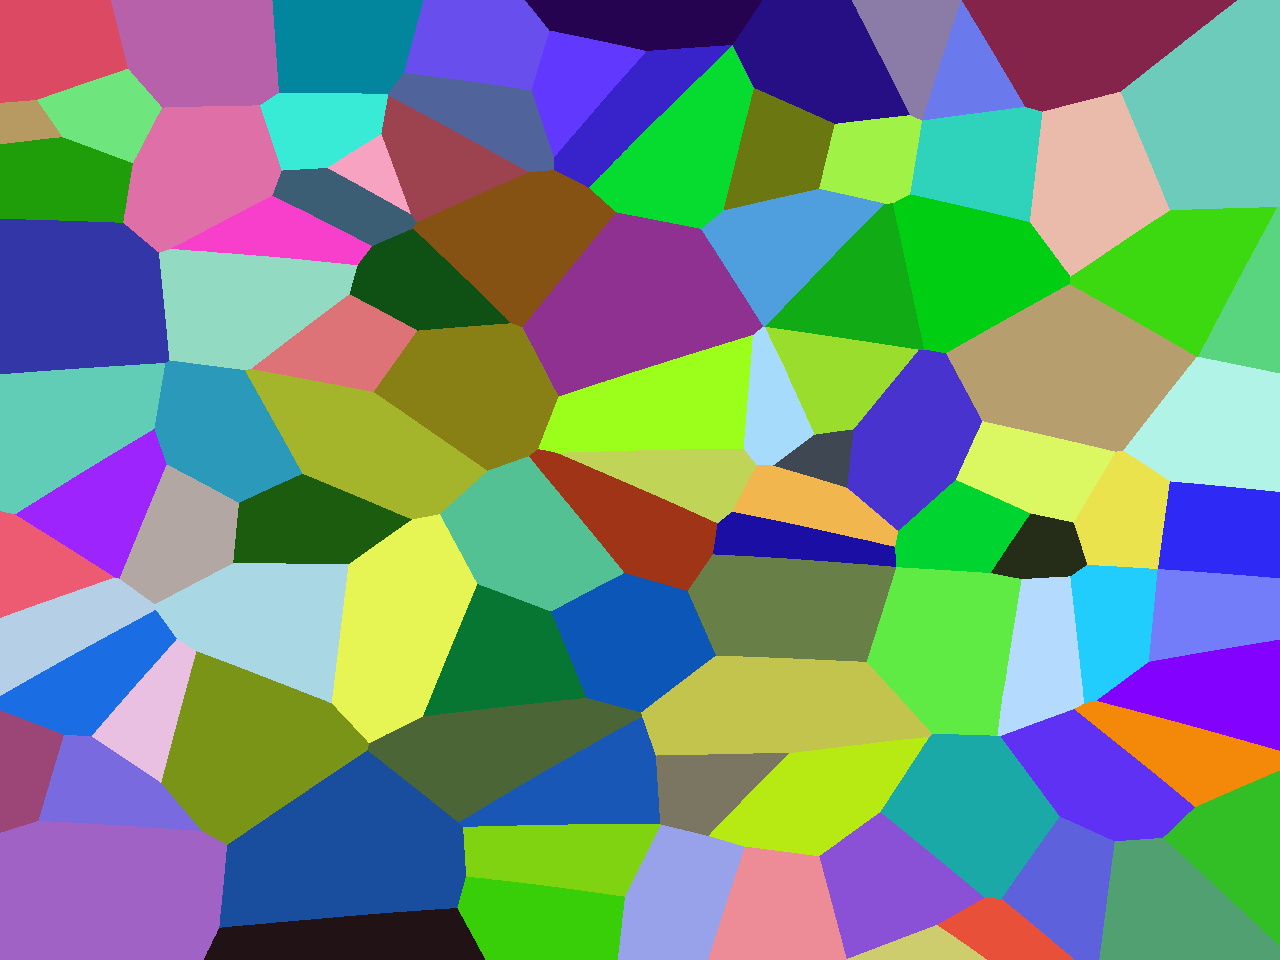
\includegraphics[width=\linewidth]{voronoi100.png}
  \caption{100 cones}\label{fig:voronoi2}
\endminipage\hfill
\minipage{0.33\textwidth}%
  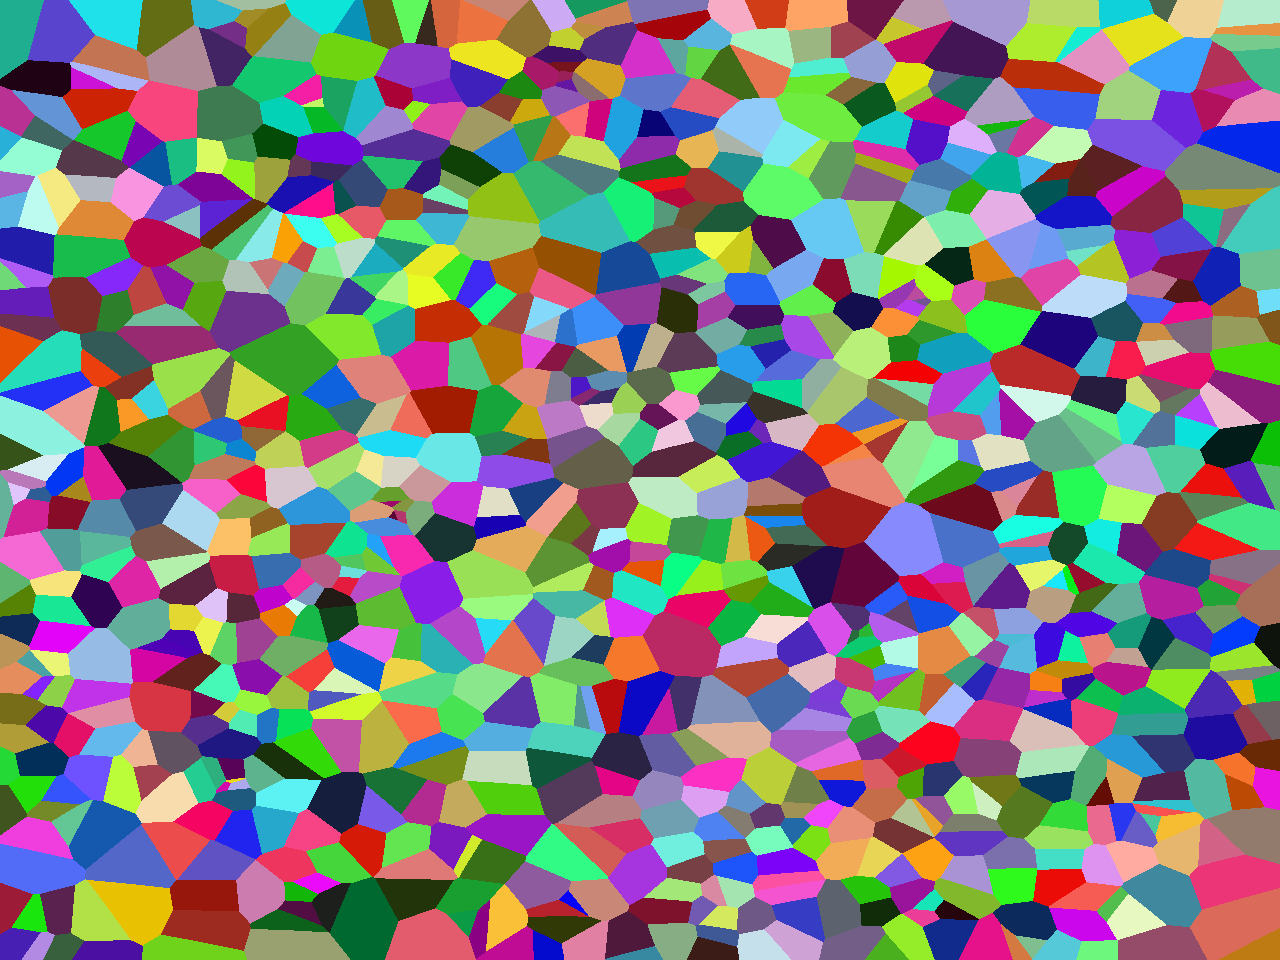
\includegraphics[width=\linewidth]{voronoi1000.png}
  \caption{1000 cones}\label{fig:voronoi3}
\endminipage
\end{figure}

\section{Thermal erosion algorithm}
\label{sec:thermalerosion}
Thermal erosion describes the process of material breaking loose due to variations in temperature during day/night cycles. This algorithm was implemented based on Jacob Olsen's description \cite{Olsen:2004}. Basically, he used a cellular automaton to model the process of thermal erosion. Cellular automata operate on grids of cells. By inspecting a cell itself and its neighborhood, one can decide how they should interact with each other. Olsen recommended to use a rotated Von Neumann neighborhood as depicted in \cref{fig:rotvonneumann}. Each of these cells correspond to heightmap tiles. If the height difference of the inspected cell and one of its neighbors is larger than a so-called talus angle $T$, material will be transported from the inspected cell to the corresponding neighbor cell as depicted in \cref{fig:thermalerosion}. This process will be repeated for all cells/tiles of the heightmap, resulting in a general smoothing of the landscape. Especially steep parts of the heightmap are most affected by this erosion process. By default Jacob Olsen's algorithm disregards material properties like hardness or softness (e.g. rock is hard, sand is soft). Therefore, as an extension of this algorithm, a way to also consider material properties will be introduced. By multiplying the amount of material to be transported by a factor that depends on the height of the inspected cell, it is possible to mimic the desired material properties.
\begin{figure}[h]
\centering
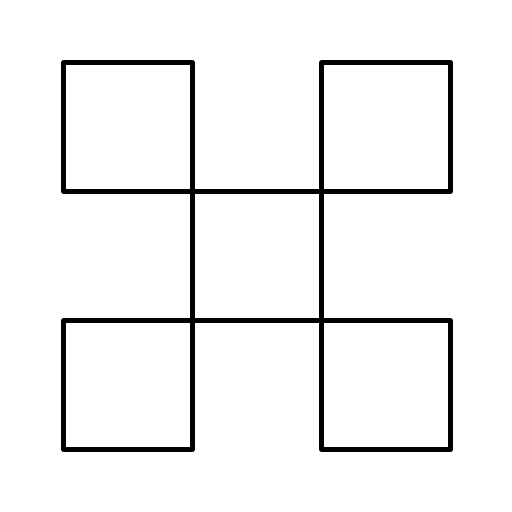
\includegraphics[width=0.25\linewidth]{rotvonneumann.png}
\caption{Rotated Von Neumann neighborhood}\label{fig:rotvonneumann}
\end{figure}

\begin{figure}[h]
\centering
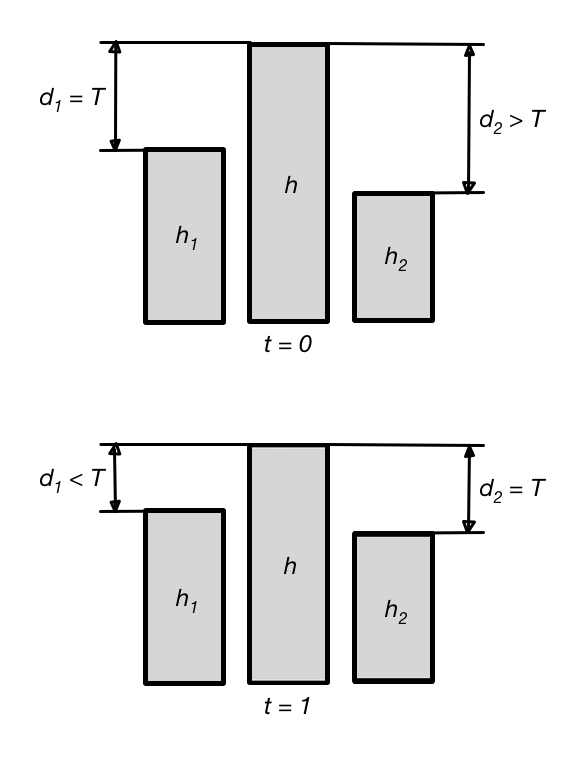
\includegraphics[width=0.5\linewidth]{thermalerosion.png}
\caption{Thermal erosion}\label{fig:thermalerosion}
\end{figure}

\section{Hydraulic erosion algorithm}
\subsection{Implementation based on previous research}
In my reasearch I came across two different papers that described how to model hydraulic erosion algorithmically. The first one \cite{Olsen:2004} was written by Jacob Olsen and featured a decent algorithm based on a cellular automaton. The idea behind this algorithm is that water (e.g. rain) causes erosion of terrain by dissolving material which gets transported by running water and once the water evaporates the material will be deposited again. To model this process it is necessary to keep track of the height-, water- as well as sediment-levels. Therefore not only a heightmap, but also a water- and sedimentmap is necessary. Each iteration can be broken down into 4 steps:

In the first step a constant amount of water is added to each cell of the watermap.

In the second step water dissolves a specific amount of material by removing material from the heightmap and adding material to the sedimentmap. A similar technique as seen in \cref{sec:thermalerosion} is used to also consider material hardness. This time around not the height but the steepness of the mountain influences the amount of material to be dissolved.

In the third step, water will transport sediment to lower altitudes. Since water is a fluid it will always try to level out meaning it will always flow from higher to lower tiles. Olsen described a cellular automaton based approach as depicted in \cref{fig:hydrolicerosion} which is capable of simulating water flow. There are 2 cases to consider. If the main cell's water level is larger than the difference of the maximum altitude $a$ (i.e. sum of cell height and water level) and the average altitude $\overline{a}$ then the excess water will be distributed among the neighboring cells while not causing them to overflow. In the other case, i.e. if the difference of $a$ and $\overline{a}$ is larger than the main cell's water level, the water of the main cell will be fully depleted and distributed evenly among the neighboring cells.

In the fourth step water will be evaporated and sediment will be deposited at its current position by lowering the cells of the water- as well as sedimentmap and raising the cells of the heightmap. The whole process will be repeated $n$ times.
\begin{figure}[h]
\centering
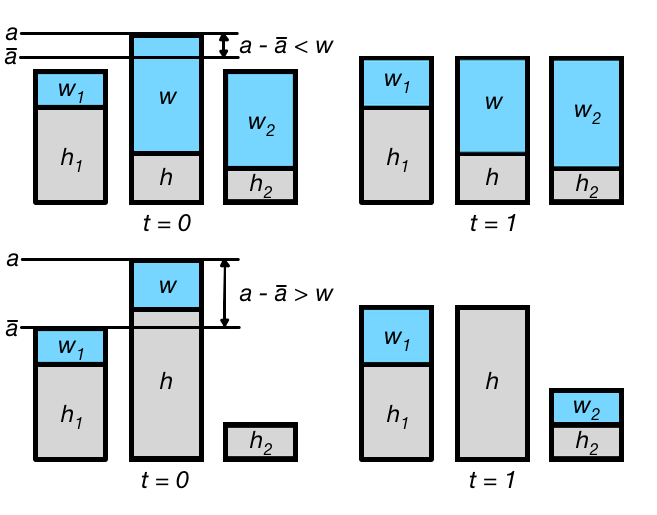
\includegraphics[width=0.65\linewidth]{hydraulicerosion.png}
\caption{Hydraulic erosion}\label{fig:hydrolicerosion}
\end{figure}
\\
\\
The second paper \cite{mei:inria-00402079} by Mei et al showcases a more advanced model of hydraulic erosion. The basic principle is still the same as described by Olsen, but Mei uses a more sophisticated water flow model which also considers fluid velocity. Due to the force of flowing water more sediment will be carried away which results in a generally more realistic model of hydraulic erosion. After studying Mei's algorithm and implementing his water flow model, a flaw in his algorithm became evident. Given that Mei's algorithm is timestep-based, it gets unstable if too large timesteps are used. Water waves begin to oscillate and ultimately the water height calculation will result in an arithmetic overflow and render the simulation unusable. To keep the simulation stable very small timesteps have to be used. In fact the timesteps required to keep the simulation stable are so small (e.g. $\Delta t = 10$ms) that one cannot even notice any difference in water flow for a couple of minutes. For a realtime application this is totally unacceptable and therefore this model was disregarded.

\subsection{Evaluation of various shallow water models}
After implementing Olsen's hydraulic erosion model and trying out various parameters it turned out that the results were not too realistic. Due to the lack of performance, the result of using Mei's variant was not too satisfying either. To achieve higher realism a more sophisticated, yet performant model had to be considered. While researching about hydraulic erosion I also stumbled upon shallow water models. These models are commonly used to predict tsunami movement but can also be utilized for other purposes like hydraulic erosion simulation. Due to the complexity at hand I was not able to implement my own shallow water model based on previous work and kept on looking for existing solutions. I found two promising projects. The first one, written in C++ by Alex Darcy, used a Riemann solver to numerically solve the shallow water equations. The only problem was that he assumed that the terrain underneath the water was perfectly flat. This might be a valid assumption for tsunami simulations but did not work for my area of application.

The second project by Trevor Dixon seemed very promising. He implemented the shallow water equations using JavaScript and Three.js framework. His code was much more readable in comparison to Alex Darcy's. The only thing missing was water ground interaction. After spending a considerable amount of time I ultimately was not able to figure out how to include this feature and went back to searching for alternatives. This is when I found out about smoothed particle hydrodynamics fluid simulations.

\subsection{Implementation based on Smoothed Particle Hydrodynamics (SPH)}
There are dozens of different existing SPH solutions out there. Most of them were proprietary and those that were not brought other issues with them like hardware incompatibility or realtime incapability. Last but not least I came across a GitHub project by Saeed Mahani. He wrote a basic SPH simulation featuring a box which gets filled up by fluid particles while obeying the laws of physics. The project was realtime capable and had no special hardware requirements. However, several alterations to the SPH simulation had to take place in order to make it usable for this project. First of all the whole visualization code had to be replaced to be compatible with the rest of my GLFW based project. After that the simulation had to be extended to also support heightmaps which it previously did not. The original code only supported planes which could not be used to model arbitrarily shaped surfaces. Due to this an alternative solution had to be implemented. My first idea was to simply add support for static (non-moving) particles and distribute them all across the heightmap. After implementing it, it became evident that this approach had several flaws. Not only were particles passing through the heightmap because of small holes inbetween the static particles, the simulation also became horribly slow due to the sheer amount of particles present in the scene. As a result a different solution had to be found. In order to make the particles appear to be influenced by the heightmap surface, some kind of force has to counteract their tending downwards movement due to gravity. To implement this kind of behaviour it is necessary to continuously check if a particle is touching the surface. A fast triangle-ray intersection test by Möller and Trumbore \cite{moller2005fast} was used to check if a particle is below the heightmap surface or not. If the intersection test indeed is positive, a short impulse in the direction perpendicular to the impact point on the heightmap surface has to be applied to the particle. Since the normals are only calculated per heightmap vertex it was necessary to approximate the impulse direction at the impact point using interpolation. Since the heightmap is rasterized into tiles it can be guaranteed that there are always 4 normals in close proximity to the impact point. These normals are normalized vectors. To get the interpolated normal from these 4 vectors one has to sum them up and normalize the result. The performance of this solution was much better than the previous one and no more particles were dropping below the surface.

Once the SPH simulation was working as intended, it was possible to utilize it to simulate a more realistic hydraulic erosion model. The idea is that each particle gets some capacity to store sediment. If a particle touches the terrain it dissolves a specific amount of it based on the predefined particle acidity. Additionally each particle has a predefined lifespan and once its time runs out it evaporates and leaves behind the sediment it carried. Heightmap changes take place if a particle dissolves sediment or if a particle evaporates. A particle potentially travels a large distance which implies that carried sediment will almost always end up somewhere distant from where it was dissolved in the first place. To simulate rain the particles will be spawned in a certain height at random positions on the xz-plane. The user can observe the simulation in realtime and experience the effects of hydraulic erosion first-hand.

\section{Tectonic plate simulation}
\label{sec:tectonicplatesimulation}
Due to the complexity of real tectonic plate movement, the design of the simulation had to be simplified to a degree which allowed it to be implemented programmatically. As a result the problem at hand was reduced to two dimensions. The general idea is to split the heightmap into several pieces, representing tectonic plates. Additionally they should be kept in motion to simulate magma flowing underneath the surface. To model this non-trivial behaviour I decided to use a physics engine. Box2D, a 2D physics engine, supports convex polygons with up to 8 vertices as well as collision detection, is very well documented and offers a test environment called \emph{testbed}. Splitting of arbitrarily shaped polygons is not supported by Box2D though. Nevertheless this engine was far superior to its alternatives in terms of documentation, community support and features. After going through the documentation and some code samples I was able to implement the missing features myself.

\subsection{Implementation using Box2D physics engine}
When working with Box2D it is very common to start off by writing a test application for \emph{testbed}. To make this test application available in \emph{testbed} it is necessary to extend the class \emph{Test} provided by Box2D and list the newly created test class in \emph{TestEntries.cpp} as specified in the Box2D documentation. The advantage of \emph{testbed} is that it provides its own visualization interface as well as several debugging options. The downside is that \emph{testbed} tests can not be used for production systems right away and have to be altered during the integration process.
Once the base test class is set up, several methods like \emph{Step}, \emph{Create}, \emph{Keyboard}, etc. provided by the super class \emph{Test} can be overwritten. \emph{Step} will be called automatically by the test environment at each timestep. \emph{Create} will be called only once and should be used to initialize variables or data structures. Method \emph{Keyboard} will be triggered each time a key is pressed. Its parameters give information about which key was pressed. To add an object to the Box2D world several steps are necessary. Firstly, a body object has to be defined. Secondly, a fixture object has to be defined and linked with the body object it corresponds to. In Box2D bodies can either be static, dynamic or kinematic. Static bodies do not move. Even if a dynamic body collides with a static body, only the dynamic body will be affected by the collision. Dynamic bodies can move and are affected by all other bodies. Kinematic bodies can also move, but are not affected by collisions caused by dynamic bodies. The tectonic plate simulation will consist of dynamic as well as kinematic bodies. The dynamic bodies will represent the tectonic plates and the kinematic bodies will be responsible for keeping the simulation in motion as well as keeping the dynamic bodies contained within the simulation area. Body objects can be used to access information like current position, angle, velocity, mass, etc. To describe the shape of a Box2D body, fixtures will be used. To define a fixture it is necessary to set the fixture's density attribute and shape. Based on the fixture's density and area it consumes, the body's mass will be determined. Box2D offers basic shapes like rectangles and circles as well as convex polygons with a maximum of 8 vertices. The tectonic plate simulation will be initialized with 5 rectangle fixtures. 4 of these will be used to define the kinematic bodies' shapes, i.e. thin beams. The last one will be used to define the dynamic body's shape, a big square. This square will be randomly split a specific amount of times during set up. Unfortunately Box2D did not offer this splitting functionality per se and it therefore had to be implemented by hand. To implement splitting of polygons it is important to know that Box2D only supports convex polygons with up to 8 vertices which need to be specified in counter clockwise winding. In order to split polygons, Box2D's raycasting feature can be very helpful. It allows the programmer to cast rays and if a ray intersects with an object a callback function will be called. When a ray is cast through a convex polygon there should always be exactly one entry point and one exit point. Box2D's raycasting only registers the first intersection point per object though. Due to this two rays had to be cast in opposite directions. Having both, the first ray's entry point and the second ray's entry point as well as all vertices the polygon consists of, the only thing left to do is to determine which vertex belongs to which slice of the polygon. The following pseudocode should adequately elaborate this procedure:
\begin{lstlisting}[caption=Point in slice check pseudocode]
entry = entry point of first ray
exit = entry point of second ray
rayCenter = ((entry.x+exit.x)/2,(entry.y+exit.y)/2)
rayAngle = atan((entry.y-exit.y)/(entry.x-exit.x))
for each vertex v of polygon:
  cutAngle = atan((v.y-rayCenter.y)/(v.x-rayCenter.x))-rayAngle
  if cutAngle < -PI:
    cutAngle += 2*PI
  if cutAngle > 0 and cutAngle <= PI:
    // vertex v belongs to polygon1
  else:
    // vertex v belongs to polygon2
\end{lstlisting}
Once the polygons (i.e. tectonic plates) are all set up, collision callbacks provided by Box2D are used to act whenever a collision occurs. For the tectonic plate simulation only the collisions between the dynamic objects, i.e. the plates, are important. Therefore the program is set up to only act on collisions in which two dynamic objects are involved. Additionally, collisions between two polygons which do not have two collision points are disregarded. By enforcing these constraints the program will only act on collisions that occur between two dynamic objects and consist of exactly two collision points. Finally, in order to use these collision points for heightmap alterations, they have to be transformed from the Box2D coordinate system to the heightmap coordinate system.

\subsection{Generation of mountain ranges due to tectonic plate collisions}
\label{subsec:generationofmountainranges}
Each tectonic plate collision results in two collision points due to the custom collision callbacks mentioned before. Using these points one can draw an imaginary line onto the heightmap. The goal would be to procedurally generate a mountain range along this imaginary line. This is where an advanced version of RMP algorithm comes into place. This version of RMP will also use a Voronoi diagram to generate arbitrary polygons. Different from the previous RMP implementation this time there will be two coordinate pairs instead of a single one. Between these coordinates Bresenham line algorithm will be performed and all colors passed will be remembered. In the next step the Voronoi diagram will be projected onto the heightmap and all heightmap vertices inside polygons that are colored with one of the remembered colors will be raised in height. This procedure will be repeated each time a tectonic plate collision occurs. As a result procedurally generated mountain ranges will arise between two colliding tectonic plates.

\section{Visualization techniques}
\subsection{Texture splatting}
Texture splatting can be used to make a computer generated terrain more visually appealing. By using textures and blending them together based on height and slope it is possible to texture procedurally generated terrain regardless of shape and complexity of terrain features. For this application four textures have been chosen:
\begin{itemize}
\item Sand
\item Grass
\item Stone
\item Snow
\end{itemize}
Blending textures together is performed by the fragment shader. The OpenGL shader language offers a function \emph{mix} that allows to linearely interpolate between two texels. \emph{Mix} consists of three parameters:
\begin{itemize}
\item First texel color
\item Second texel color
\item A floating-point number between 0.0 and 1.0 representing the mixture ratio
\end{itemize}
\begin{lstlisting}[caption=Fragment shader texture chooser pseudocode]
color0 = sand texture
color1 = grass texture
color2 = rock texture
color3 = snow texture

max_height = max height of terrain
min_height = min height of terrain

difference = max_height-min_height
delta = difference / 4
threshold0 = delta*1
threshold1 = delta*2
threshold2 = delta*3

position = pass-through position from vertex shader

if position.y < threshold0:
  texel = color0
if position.y >= threshold0 and position.y < threshold0+delta):
  texel = mix(color0, color1, (position.y-threshold0)/delta)
if position.y >= threshold0+delta and position.y < threshold1):
  texel = color1
// the remaining textures are blended similarily...
\end{lstlisting}
Up to now only the height information is used to determine which texture should be applied on the terrain. Of course this model does not look too realistic since the slope information has not been considered so far. Grass does not grow on steep slopes. Same goes for snow. Snow will only be at rest on flat areas. Therefore in steep slopes grass and snow texels have to be overridden by rock texels. A common approach to determine the steepness of a slope is to use the normal vectors' y coordinates. Using thresholds it is again possible to utilize OpenGL's \emph{mix} function to mix two texels. Unfortunately there are some special cases, namely steep slopes inside an area between two height thresholds which required bilinear interpolation instead of linear interpolation. These cases were solved by calling \emph{mix} in a nested way, meaning the first or second parameter of \emph{mix} is itself the result of a previous \emph{mix} invocation.

\subsection{Bloom shader effect}
A bloom shader effect is a popular choice to enhance the realism of a scene. The goal is to reproduce image imperfections caused by real-world cameras. Brightly lit spots often appear to be glowing when captured with a camera. To model this effect two filters are necessary:
\begin{itemize}
\item Bright-pass filter
\item Blur filter
\end{itemize}
The bright-pass filter will be applied to the original frame. After that the result will be blurred using a blur filter, e.g. a two-pass Gaussian filter. Finally the original frame as well as the blurred bright-pass frame will be blended together resulting in an image with brightly glowing regions. Altogether the bloom filter consists of 5 rendering passes:
\begin{enumerate}
  \item Normal scene render pass (\cref{fig:1stpass})
  \item Bright-pass (\cref{fig:2ndpass})
  \item Horizontal Gauss blur pass (\cref{fig:3rdpass})
  \item Vertical Gauss blur pass (\cref{fig:4thpass})
  \item Bloom pass (\cref{fig:5thpass})
\end{enumerate}

\begin{figure}[!htb]
\minipage{0.33\textwidth}
  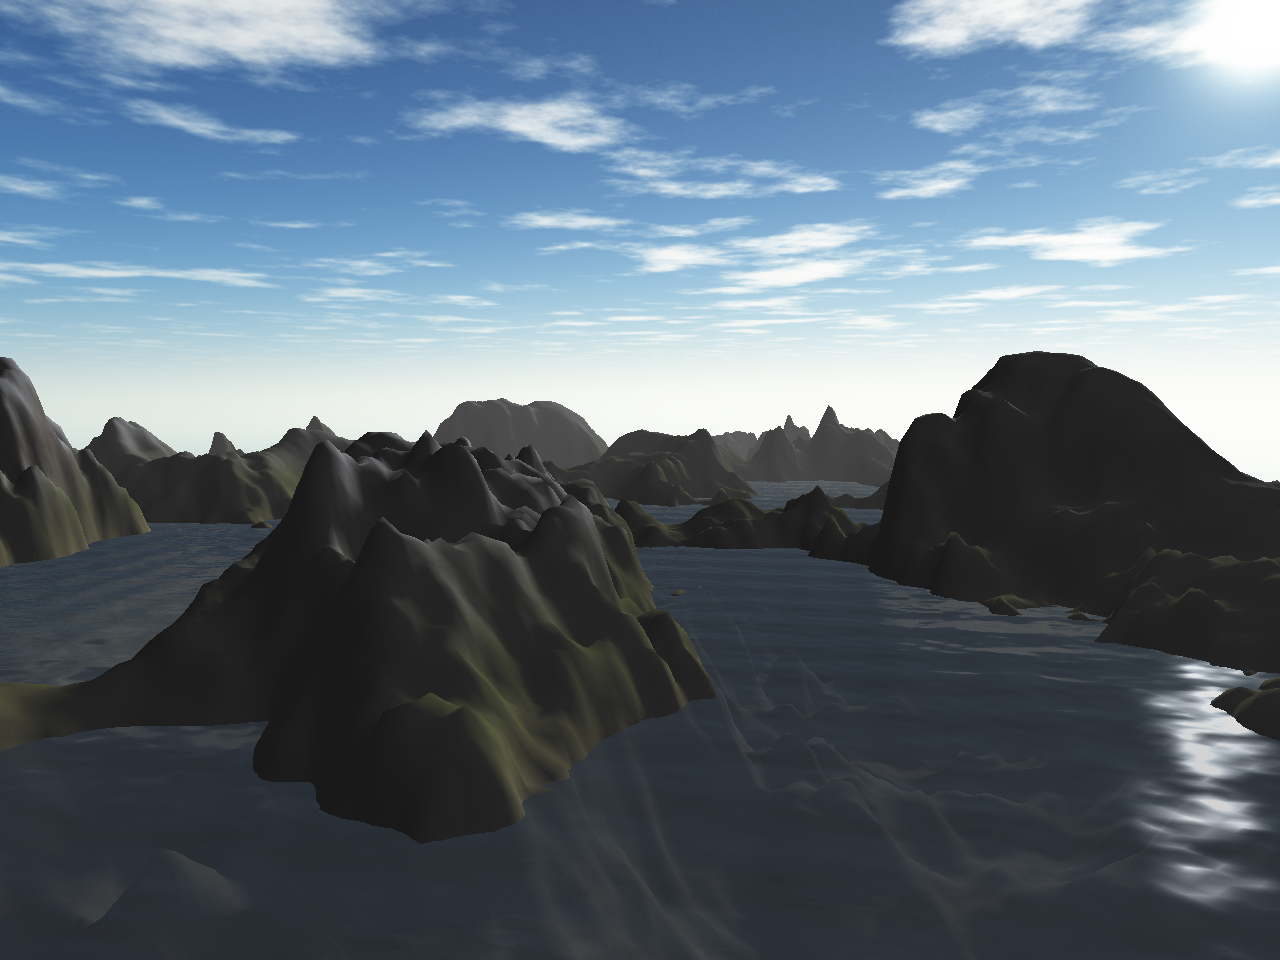
\includegraphics[width=\linewidth]{shader0-no-effect-screenshot.png}
  \caption{Normal scene render pass}\label{fig:1stpass}
\endminipage\hfill
\minipage{0.33\textwidth}
  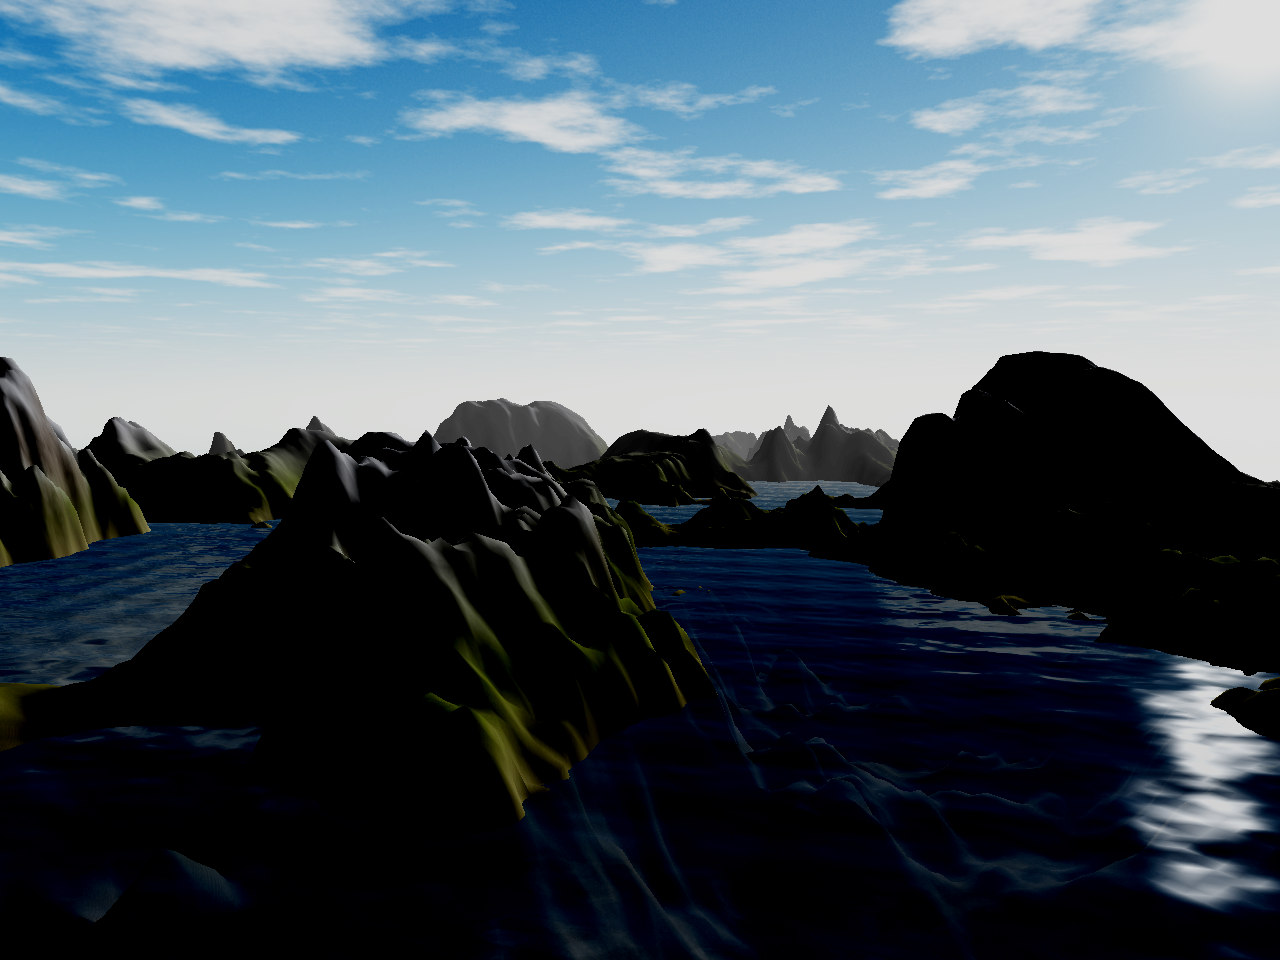
\includegraphics[width=\linewidth]{shader1-brightpass-screenshot.png}
  \caption{Bright-pass filter pass}\label{fig:2ndpass}
\endminipage\hfill
\minipage{0.33\textwidth}%
  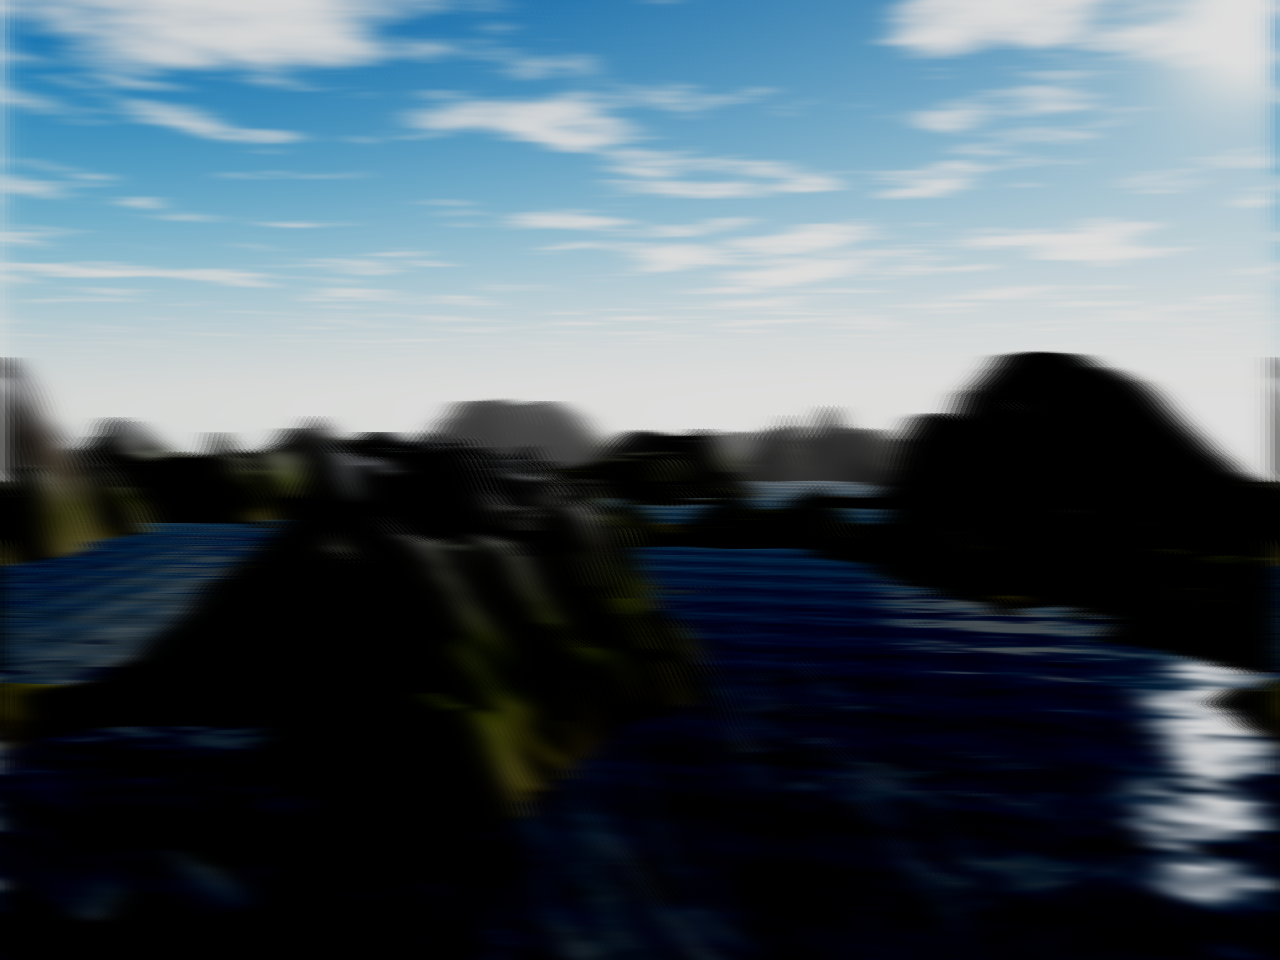
\includegraphics[width=\linewidth]{shader2-horizontal-blur-screenshot.png}
  \caption{Horizontal Gauss blur pass}\label{fig:3rdpass}
\endminipage
\\
\centering
\minipage{0.33\textwidth}
  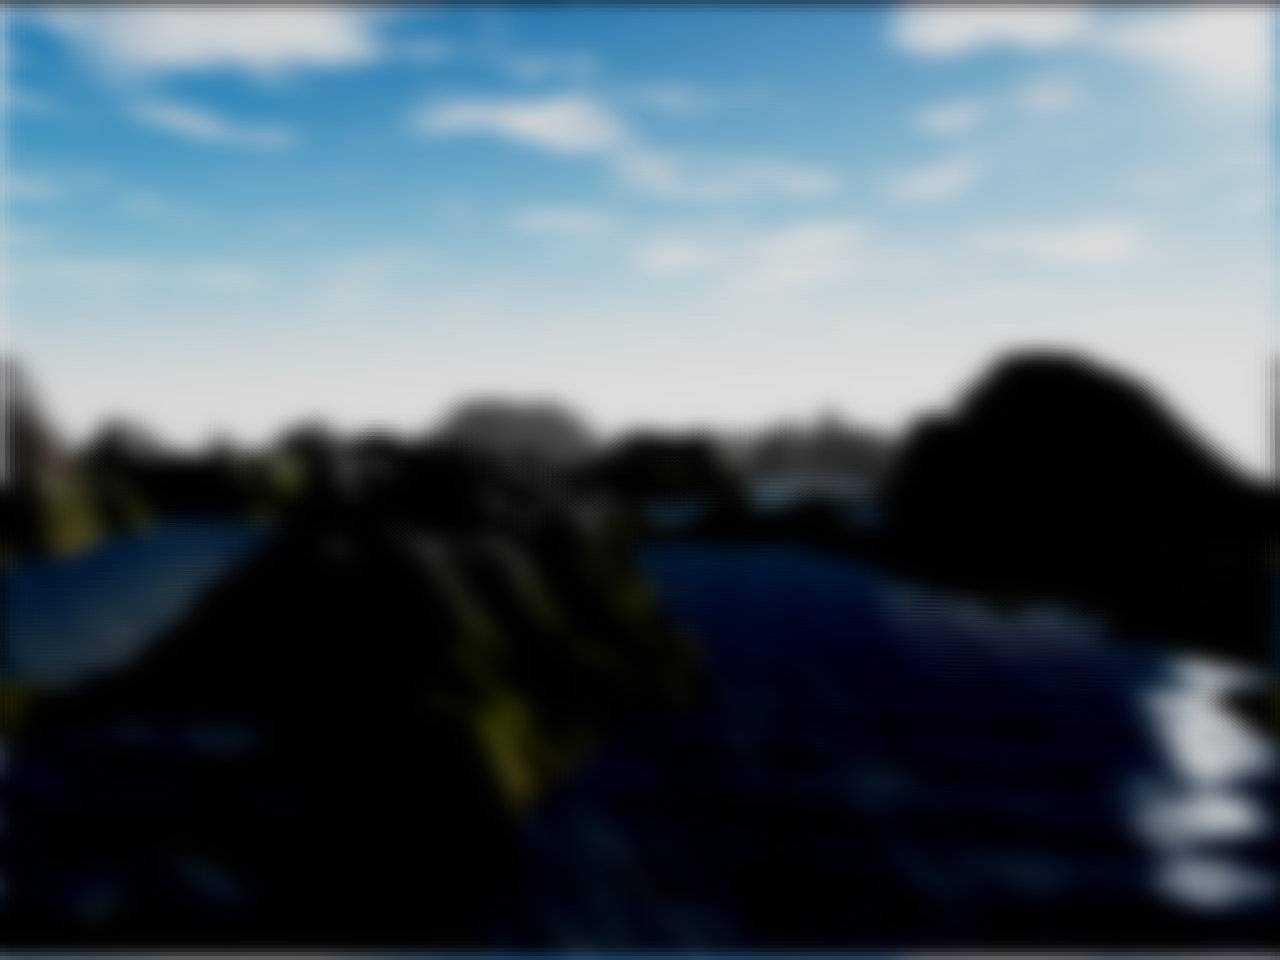
\includegraphics[width=\linewidth]{shader3-vertical-blur-screenshot.png}
  \caption{Vertical Gauss blur pass}\label{fig:4thpass}
\endminipage
\minipage{0.005\textwidth}
\
\endminipage
\minipage{0.33\textwidth}%
  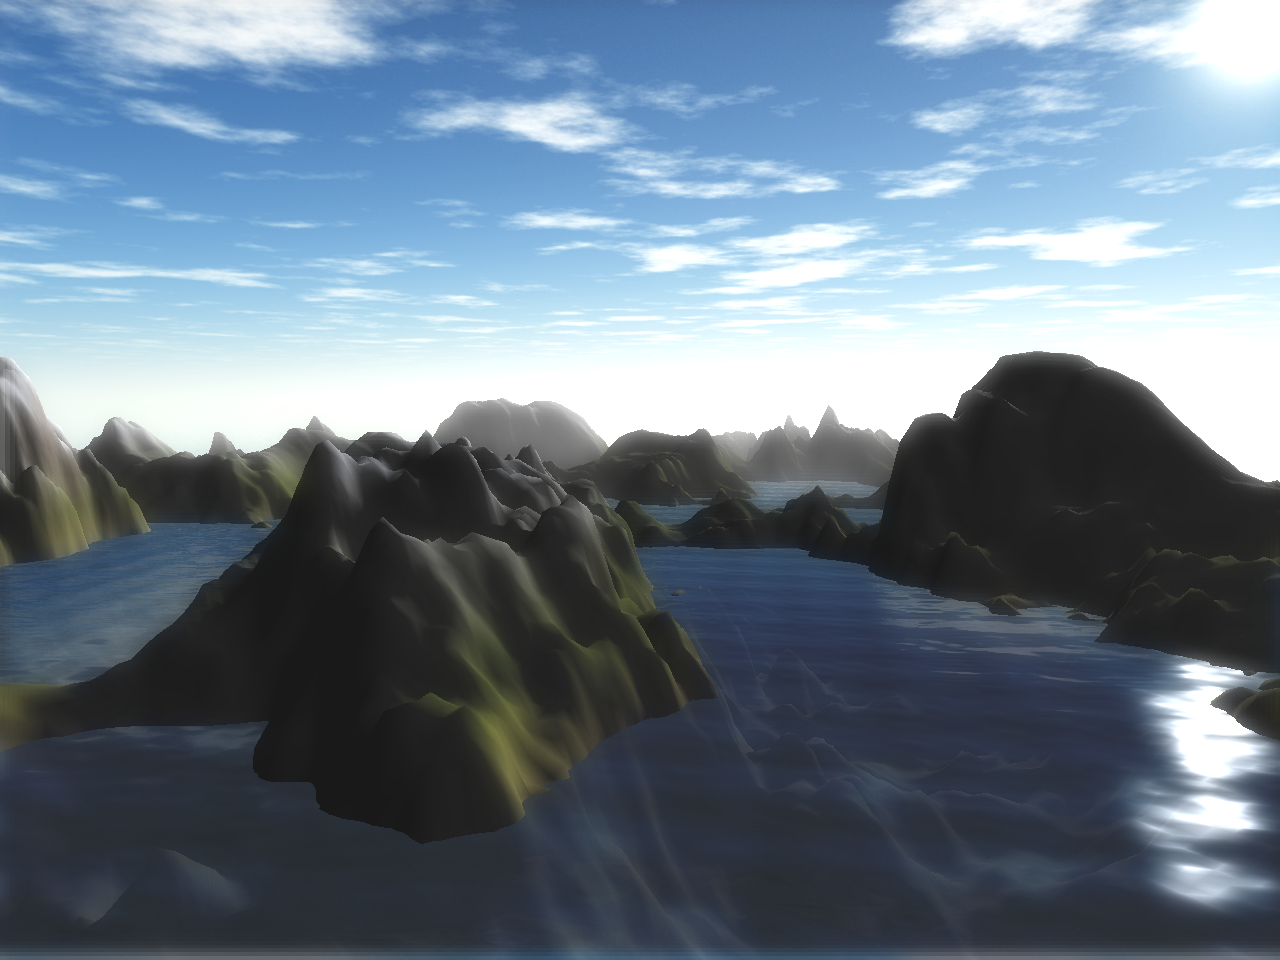
\includegraphics[width=\linewidth]{shader4-bloom-screenshot.png}
  \caption{Bloom shader pass}\label{fig:5thpass}
\endminipage
\end{figure}

\subsubsection{Bright-pass filter}
This filter makes bright regions even brighter while not modifying dark regions. It is possible to specify the range of colors to be brightened as well as the amount they should be brightened by. The bright-pass shader code is based on Erik Reinhard's formula:
\begin{align*}
L_d(x,y) = \frac{L(x,y) * \frac{1 + L(x,y)}{L_{white}^2}}{1 + L(x,y)}
\end{align*}
which can be found in his paper \cite{Reinhard:2002:PTR:566570.566575}.

\subsubsection{Two-pass Gaussian filter}
A two-pass Gaussian filter consists of two passes, namely a horizontal and a vertical Gaussian blur pass. During these passes each pixel will be averaged using a one-dimensional Gaussian kernel. The two-pass Gaussian filter is computationally less expensive than the one-pass Gaussian filter using a two-dimensional Gaussian kernel. For this filter the vertex shader is responsible for setting up the pixel coordinates to be averaged by the fragment shader based on Gauss distributed weights.
\\
Vertex shader pseudocode:
\begin{lstlisting}[caption=Two-pass Gaussian filter vertex shader]
UV = input pixel location
direction = (1,0) or (0,1) depending on pass direction
offsets[] = one-dimensional Gaussian kernel

for i between 0 and offsets.length:
  blurUV[i] = UV+(direction.x*offsets[i],direction.y*offsets[i])
\end{lstlisting}
Fragment shader pseudocode:
\begin{lstlisting}[caption=Two-pass Gaussian filter fragment shader]
texture = input frame
blurUV[] = array of input pixel locations to be averaged
weights[] = array of Gauss distributed values based on kernel

color = (0,0,0) // output color

for i between 0 and weights.length:
  color += texture.pixelAt(blurUV[i])*weights[i]
\end{lstlisting}

\subsection{Exporting heightmaps}
\label{subsec:exportingheightmaps}
Obviously, once an interesting heightmap has been generated it is desireable to save it for future usage. To generate heightmaps that are compatible with the huge variety of tools available, it is necessary to choose a common file format. Research shows that most programs that work with heightmaps (e.g. Terragen) support 8-bit grayscale images using .png file format. It is important to note that 8-bit images allow only a maximum of 256 different height levels. For small heightmaps with equal or less than 512x512 tiles this is more than enough. Each pixel of the grayscale image will be used to store vertex y-coordinates.
\begin{figure}[h]
\centering
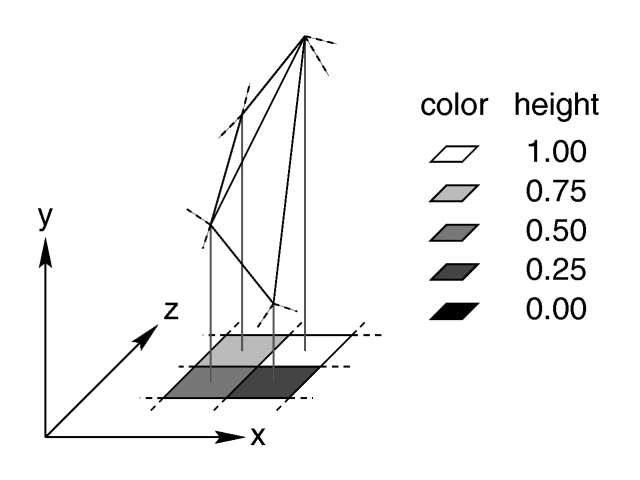
\includegraphics[width=0.4\linewidth]{pixhfld.png}
\caption{
  Simplified heightmap export process \cite{POVRay:HeightField}
}
\label{fig:heightfield}
\end{figure}
\Cref{fig:heightfield} depicts this process for a 1x1 heighmap. There are some special cases to consider which would result in invalid heightmap exports if not handled properly:
\begin{itemize}
  \item Heightmaps containing vertices with negative y-coordinates
  \item Heightmaps containing vertices with y-coordinates exceeding the upper bound
\end{itemize}
These problems can be resolved by translating and scaling the heightmap along the y-axis in a way that satisfies both requirements. The following pseudo-code shows how this issue was dealt with programmatically:
\begin{lstlisting}[caption=Heightmap export pseudo-code]
imageWidth = hm.getColumns() + 1
imageHeight = hm.getRows() + 1
image[] = array of length imageWidth*imageHeight

for y between 0 and imageHeight:
  for x between 0 and imageWidth:
    image[y*imageWidth + x] = ((hm.getHeightAt(x,y) - hm.getMinHeight()) / (hm.getMaxHeight() - hm.getMinHeight())) * 256
\end{lstlisting}

\subsection{Capturing screenshots with stblib}
OpenGL provides a function called glReadPixels which copies a specified region of pixels from the video card memory to the RAM. RGB images require width * height * 3 bytes per pixel. Since a char requires exactly one byte of space it is commonly used to represent color channel information. In fact a library called stblib written by Sean T. Barret et al is perfectly capable of saving these kinds of character arrays in various file formats like .jpg or .png and was used for this purpose.

\subsection{Video recording with ffmpeg}
To efficiently record a video it is necessary to allocate enough space beforehand. Reallocating space during the capturing process leads to noticeable stuttering and is not an option. The following formula was used to calculate the amount of required space:
\begin{align*}
space(width, height, fps, t) = width * height * 3 * fps * t \; \mathrm{bytes}
\end{align*}
Using OpenGL's glReadPixels function it was possible to save each frame into an array of type char. Once all the frames are captured they need to be encoded using ffmpeg's MPEG2 encoding algorithm. Therefore each frame has to be converted from RGB to YCbCr color space using ffmpeg library. For some reason ffmpeg's YCbCr color conversion algorithm flips the frame vertically during conversion. After flipping the frame back it is ready to be encoded by ffmpeg. Once all frames are encoded, ffmpeg will save the video as .mpg file on the harddisk. The file format .mpg can be played with almost any video player and does not require too much space due to MPEG2 encoding algorithm provided by ffmpeg.

%----------------------------------------------------------------------------------------
\chapter{Results}
\label{sec:results}

\section{Comparison of hydraulic erosion algorithms}
The algorithms being compared are Jacob Olsen's cellular automata based approach as well as the SPH based alternative. Both algorithms were applied to predefined heightmap surfaces of different shapes for 10 minutes each. The shapes in concern are
\begin{itemize}
\item a crooked surface
\item a pyramid-like surface
\item a hemispheric surface
\end{itemize}
Although Olsen's algorithm showed consistent results independently of the shape it was applied to, the results were quite unspectacular.
\begin{figure}[!htb]
\minipage{0.33\textwidth}
  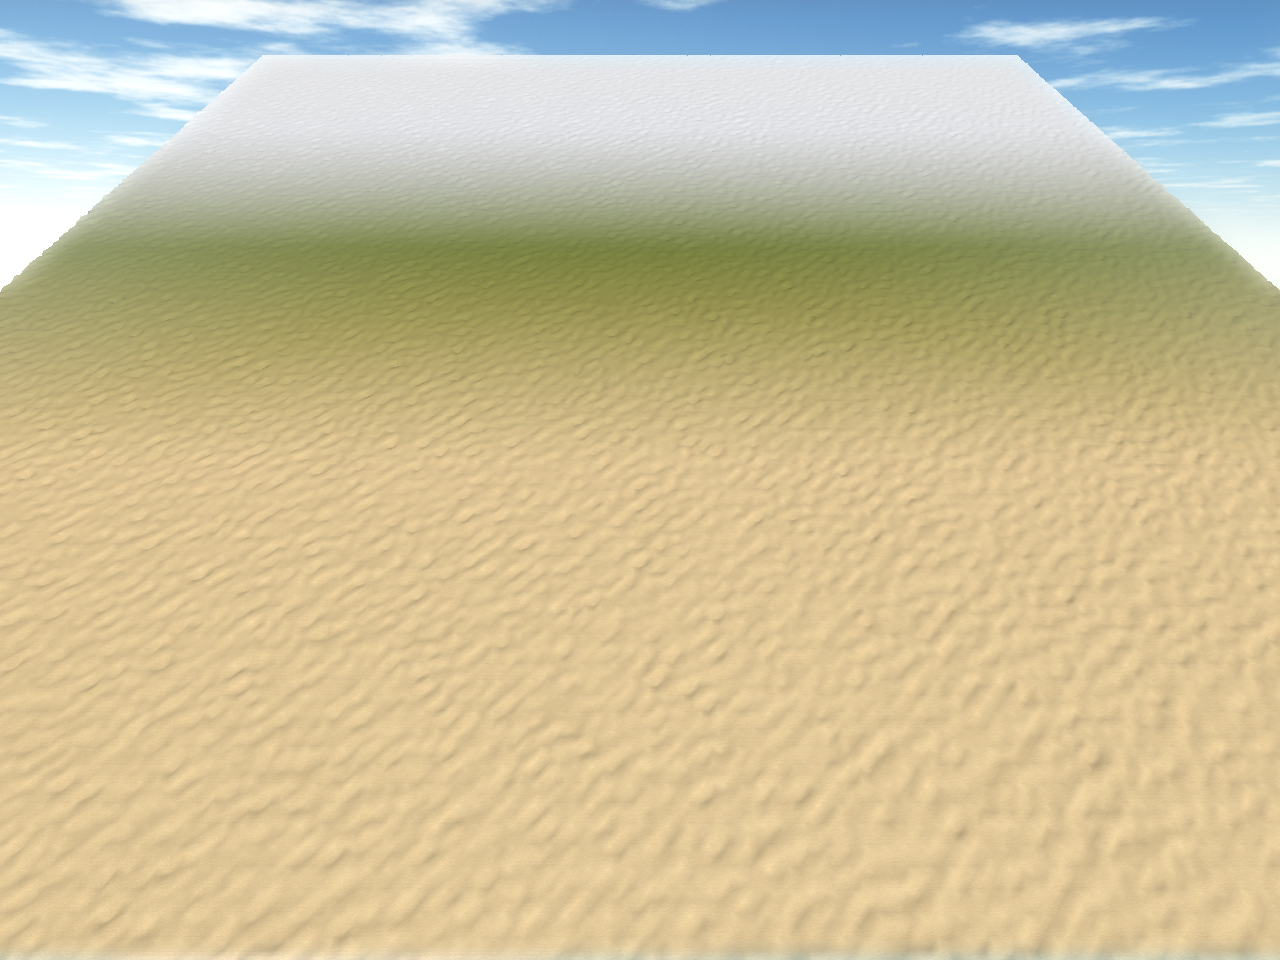
\includegraphics[width=\linewidth]{hydro-10mins-46k-iterations-crooked.png}
  \caption{Crooked surface eroded by cellular automata based hydraulic erosion}\label{fig:hydro1}
\endminipage\hfill
\minipage{0.33\textwidth}
  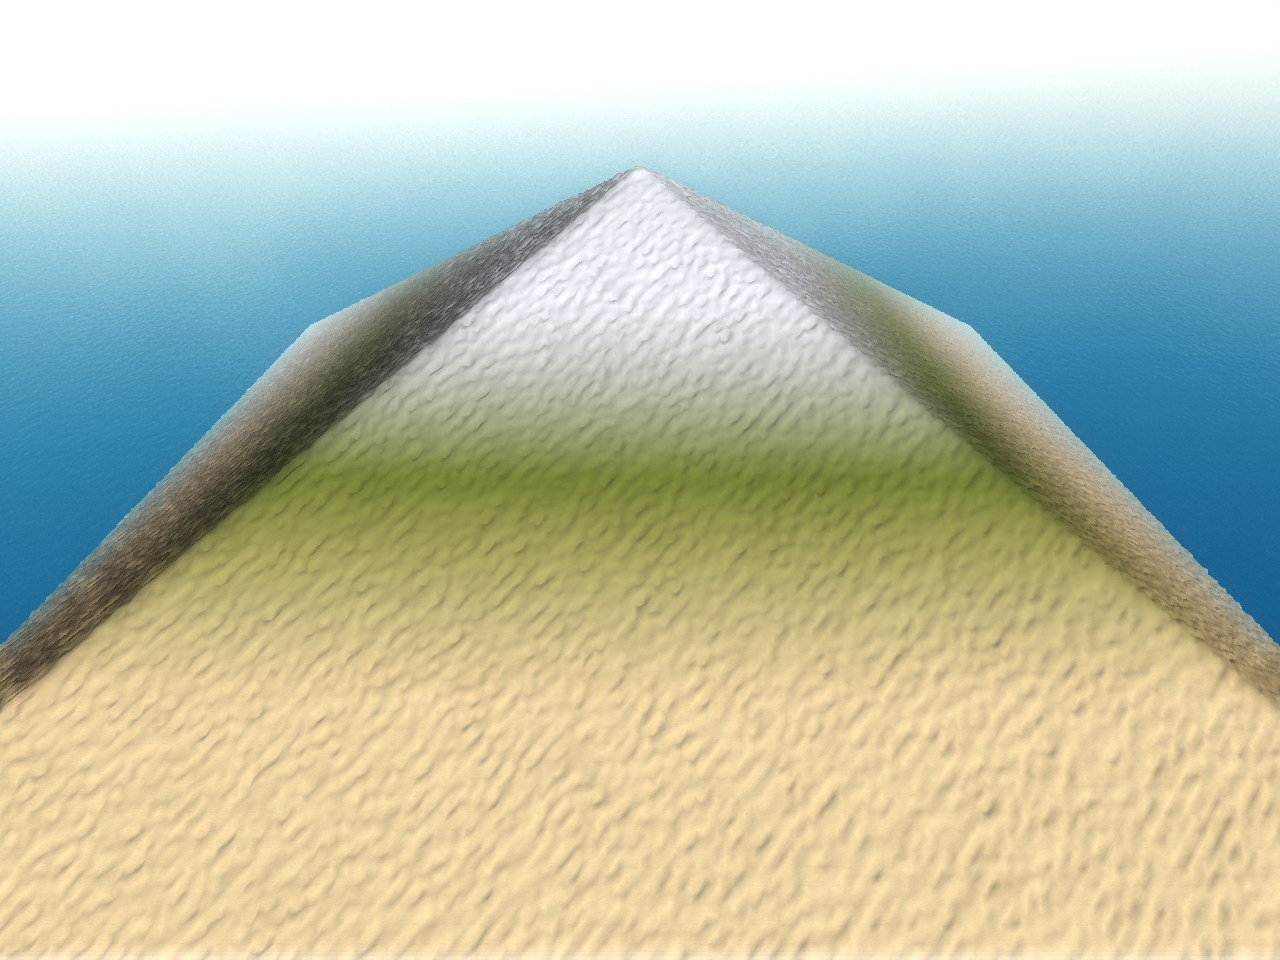
\includegraphics[width=\linewidth]{hydro-10mins-46k-iterations-pyramid.png}
  \caption{Pyramid surface eroded by cellular automata based hydraulic erosion}\label{fig:hydro2}
\endminipage\hfill
\minipage{0.33\textwidth}%
  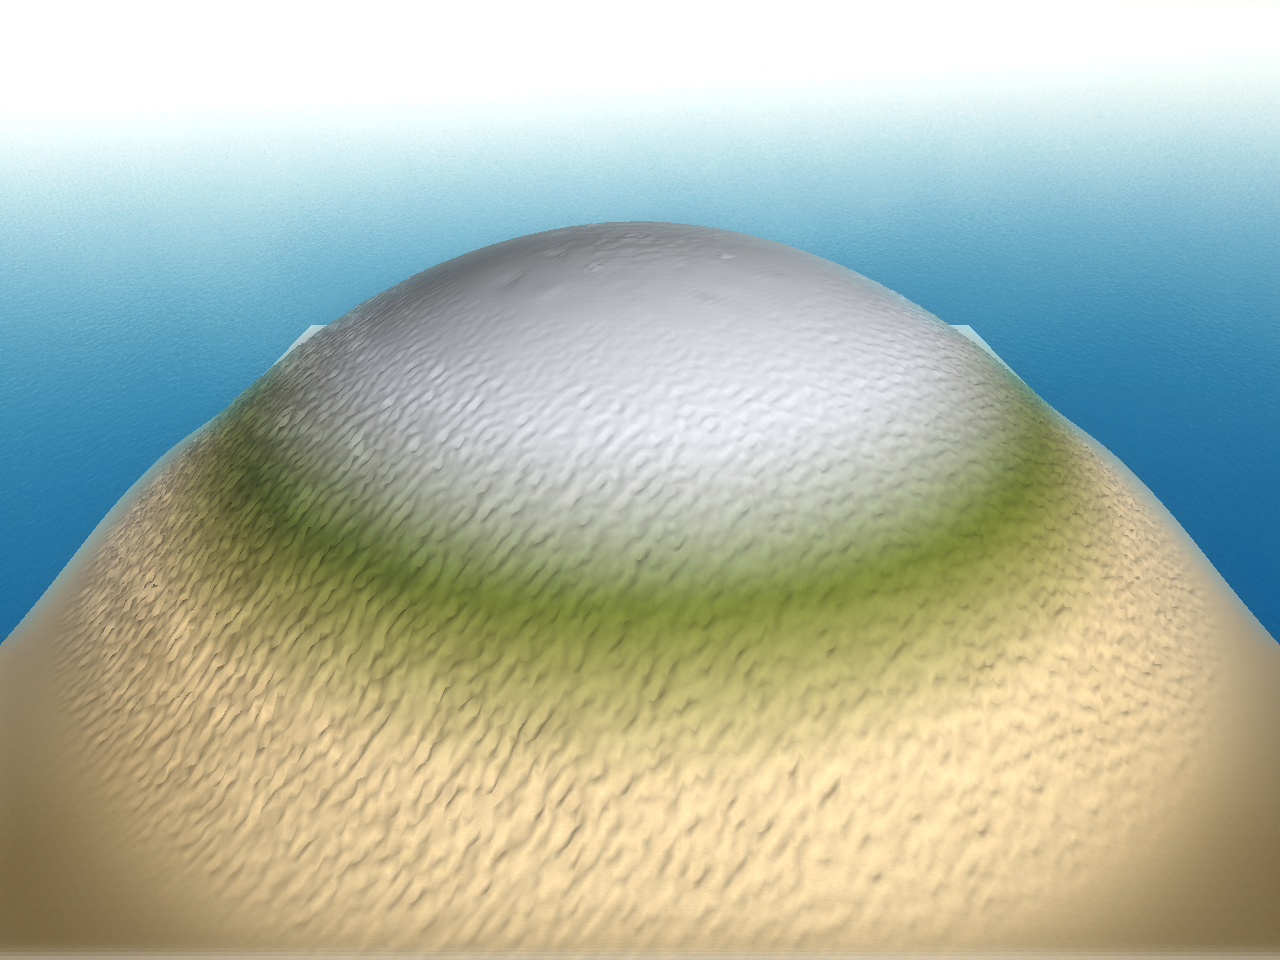
\includegraphics[width=\linewidth]{hydro-10mins-46k-iterations-hemisphere.png}
  \caption{Hemispheric surface eroded by cellular automata based hydraulic erosion}\label{fig:hydro3}
\endminipage
\end{figure}
\Cref{fig:hydro1,fig:hydro2,fig:hydro3} depict Olsen's algorithm applied to the shapes mentioned beforehand. All ditches measured about the same width and depth and did look very unoriginal. Performing the experiment several times beared the same surface transformations in each iteration. The SPH based approach on the other hand showed very promising results. Firstly, the shape the algorithm was applied to, directly influenced the erosion process. Secondly, the generated ditches had different widths and depths each. Performing the experiment several times resulted in totally different surface transformations. This is due to the fact that the SPH based approach simulates real particle movement while Olsen's approach is an abstract model based on cellular automata and does not consider flow velocity.
\begin{figure}[!htb]
\minipage{0.33\textwidth}
  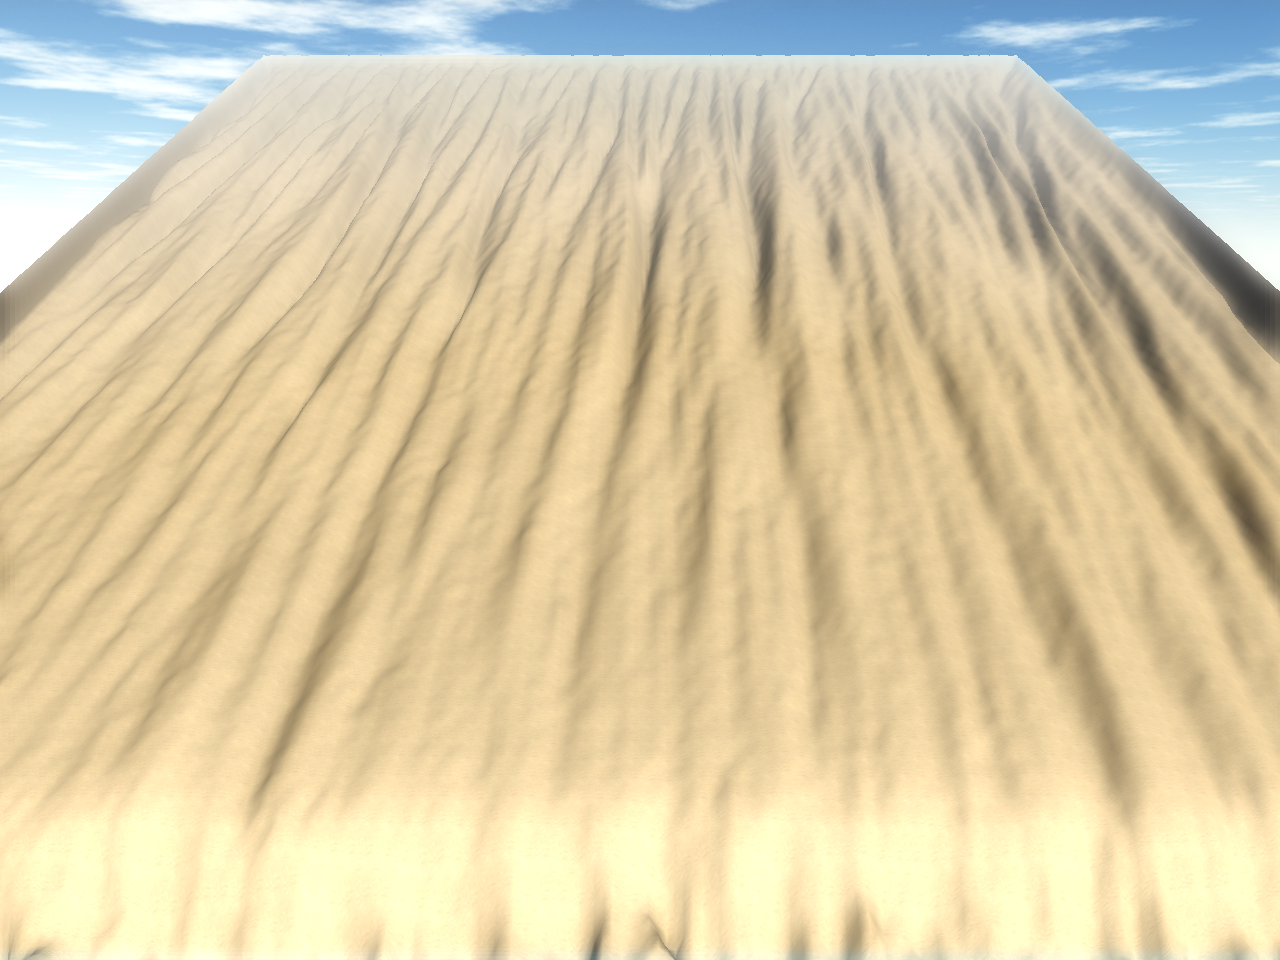
\includegraphics[width=\linewidth]{sph-hydro-10mins-crooked.png}
  \caption{Crooked surface eroded by SPH-based hydraulic erosion}\label{fig:hydro4}
\endminipage\hfill
\minipage{0.33\textwidth}
  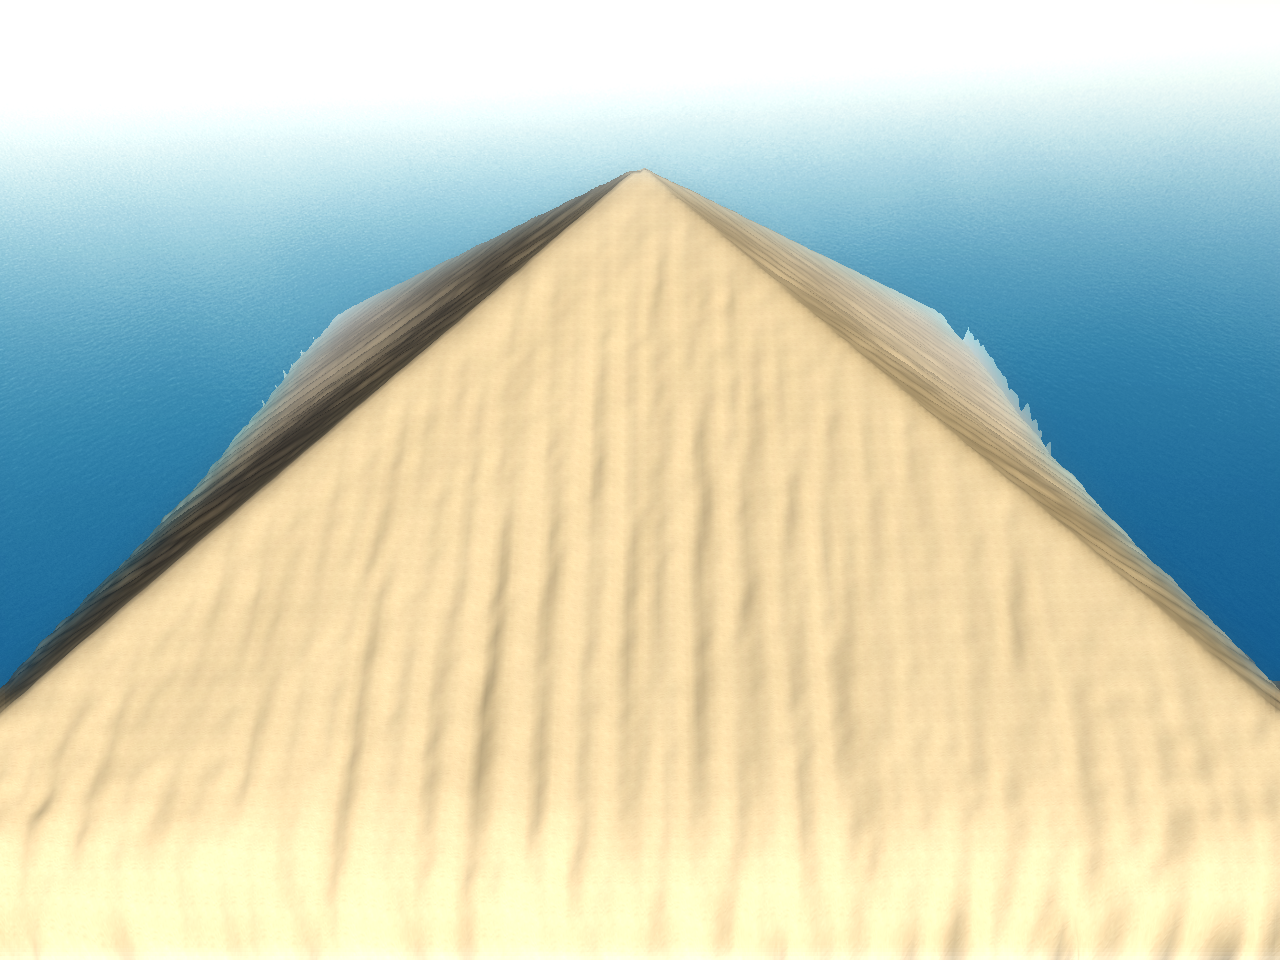
\includegraphics[width=\linewidth]{sph-hydro-10mins-pyramid.png}
  \caption{Pyramid surface eroded by SPH-based hydraulic erosion}\label{fig:hydro5}
\endminipage\hfill
\minipage{0.33\textwidth}%
  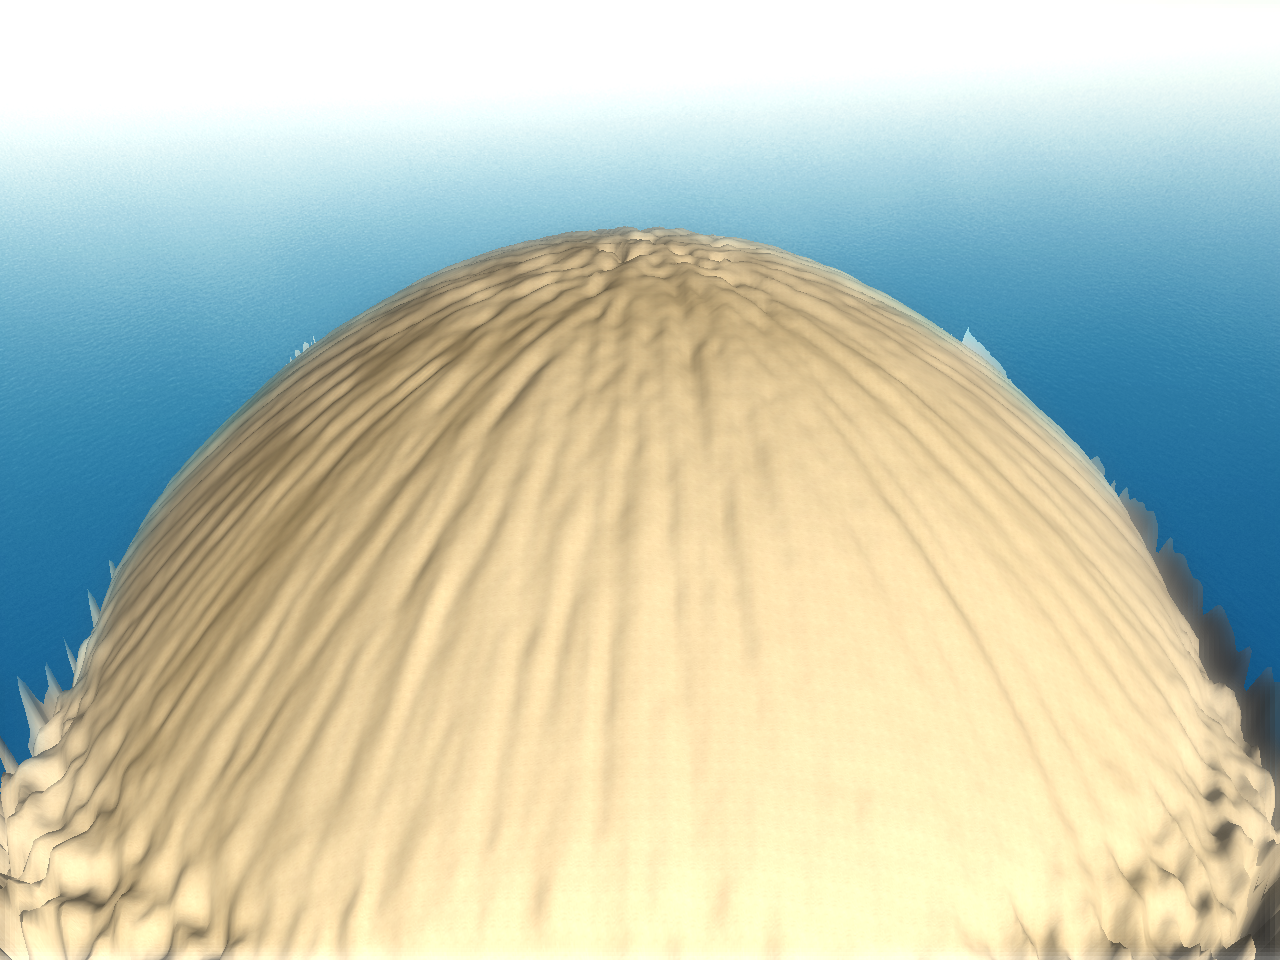
\includegraphics[width=\linewidth]{sph-hydro-10mins-hemisphere.png}
  \caption{Hemispheric surface eroded by SPH-based hydraulic erosion}\label{fig:hydro6}
\endminipage
\end{figure}
\Cref{fig:hydro4,fig:hydro5,fig:hydro6} depict the SPH based algorithm applied to the shapes mentioned beforehand. Concluding this experiment, it is evident that utilizing SPH simulations for hydraulic erosion algorithms bears very promising results. SPH simulations are capable of modelling fluid flow velocity autonomously. This behavior substantially influences the realism of the hydraulic erosion process and therefore, SPH simulations should be preferred over cellular automata when it comes to modelling hydraulic erosion.

\section{Mountain range generation algorithm alterations}
The mountain range generation algorithm is a major component of the tectonic plate algorithm as described in \cref{subsec:generationofmountainranges}. It uses a modified version of Voronoi-based RMP algorithm in order to procedurally generate mountain ranges. By extracting the mountain range generation portion from the tectonic plate algorithm and removing the randomness of tectonic plate movement it was possible to reliably conduct an experiment. The goal for this experiment was to determine if slight alterations in the mountain range generation code, namely dynamic instead of static areal height assignments, would result in higher realism. \Cref{fig:voronoi2diagonal} might help to understand what the experiment is all about. Instead of raising the whole bordered area, the goal is to raise each colored area inside the border individually. The experiment consisted of two iterations. To determine if the alterations had any effect, a control experiment was performed using the unaltered code as depicted in \cref{fig:mountainrangenormal}. \Cref{fig:mountainrangealteration} shows the final result after the alterations. Unfortunately the effect of the alterations is very subtle. While the control experiment showed no variation in mountain top elevation, the alterated version of the algorithm produced mountain tops that slightly vary in height. Even though the effects only were very subtle, the alterations still were merged into the original mountain range generation code since they had no impact performance-wise while still contributing to the realism of the scene.

\begin{figure}[!htb]
\minipage{0.33\textwidth}
  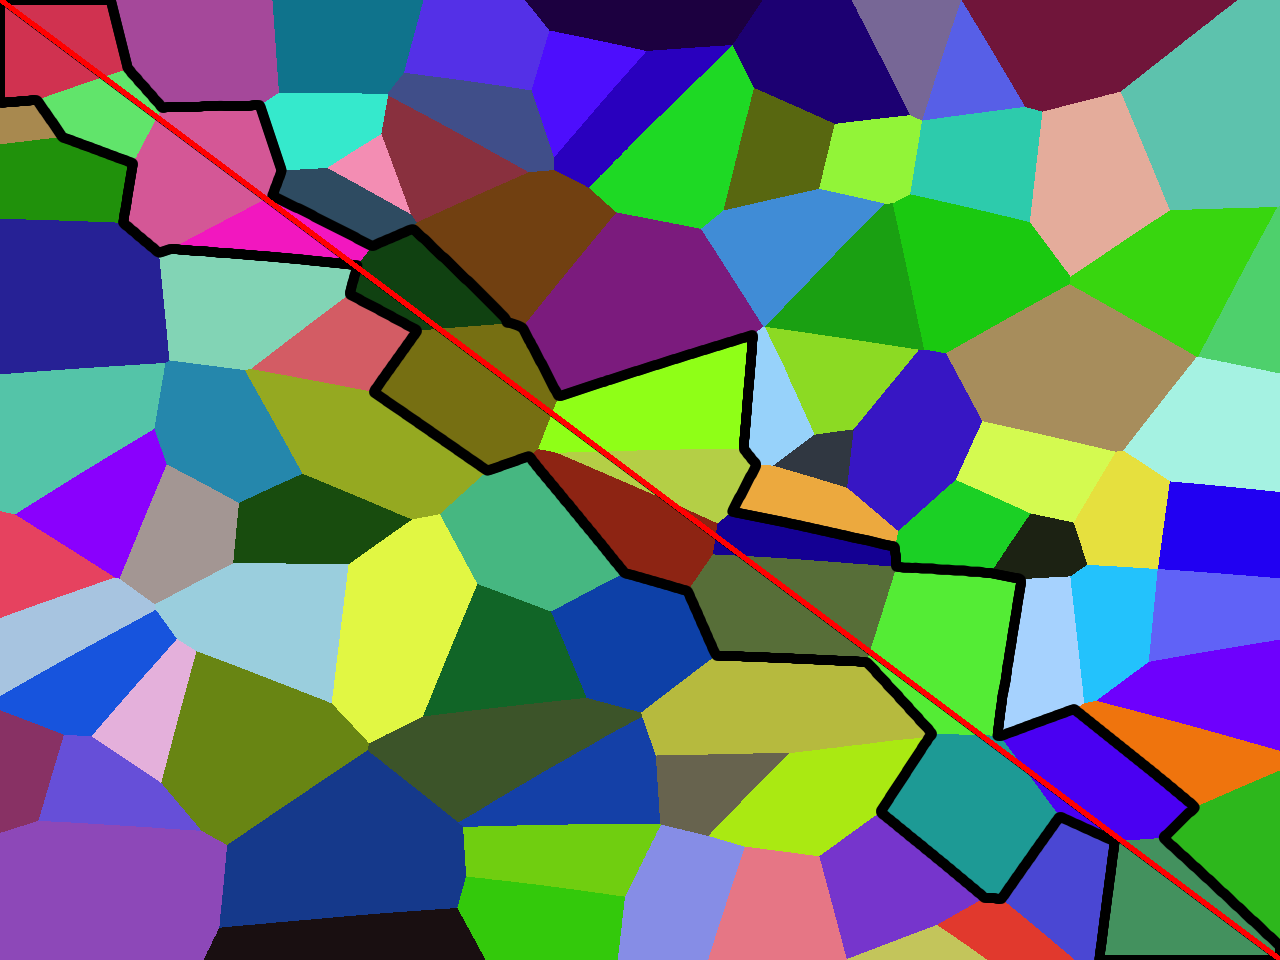
\includegraphics[width=\linewidth]{voronoi100-diagonal.png}
  \caption{Visualization of the experiment}\label{fig:voronoi2diagonal}
\endminipage\hfill
\minipage{0.33\textwidth}
  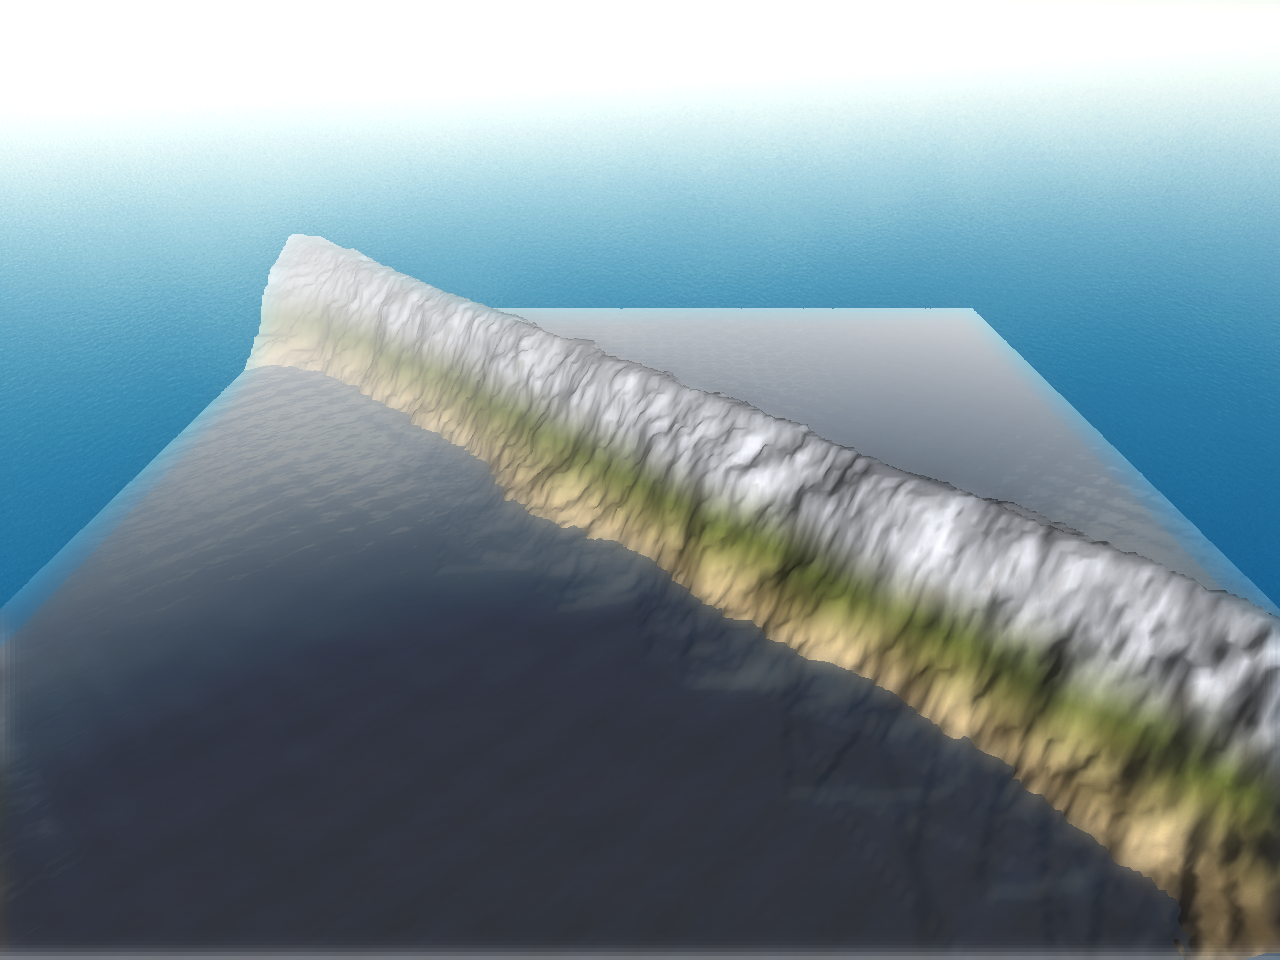
\includegraphics[width=\linewidth]{mountain-range-normal.png}
  \caption{Each affected area raised by the same amount}\label{fig:mountainrangenormal}
\endminipage\hfill
\minipage{0.33\textwidth}%
  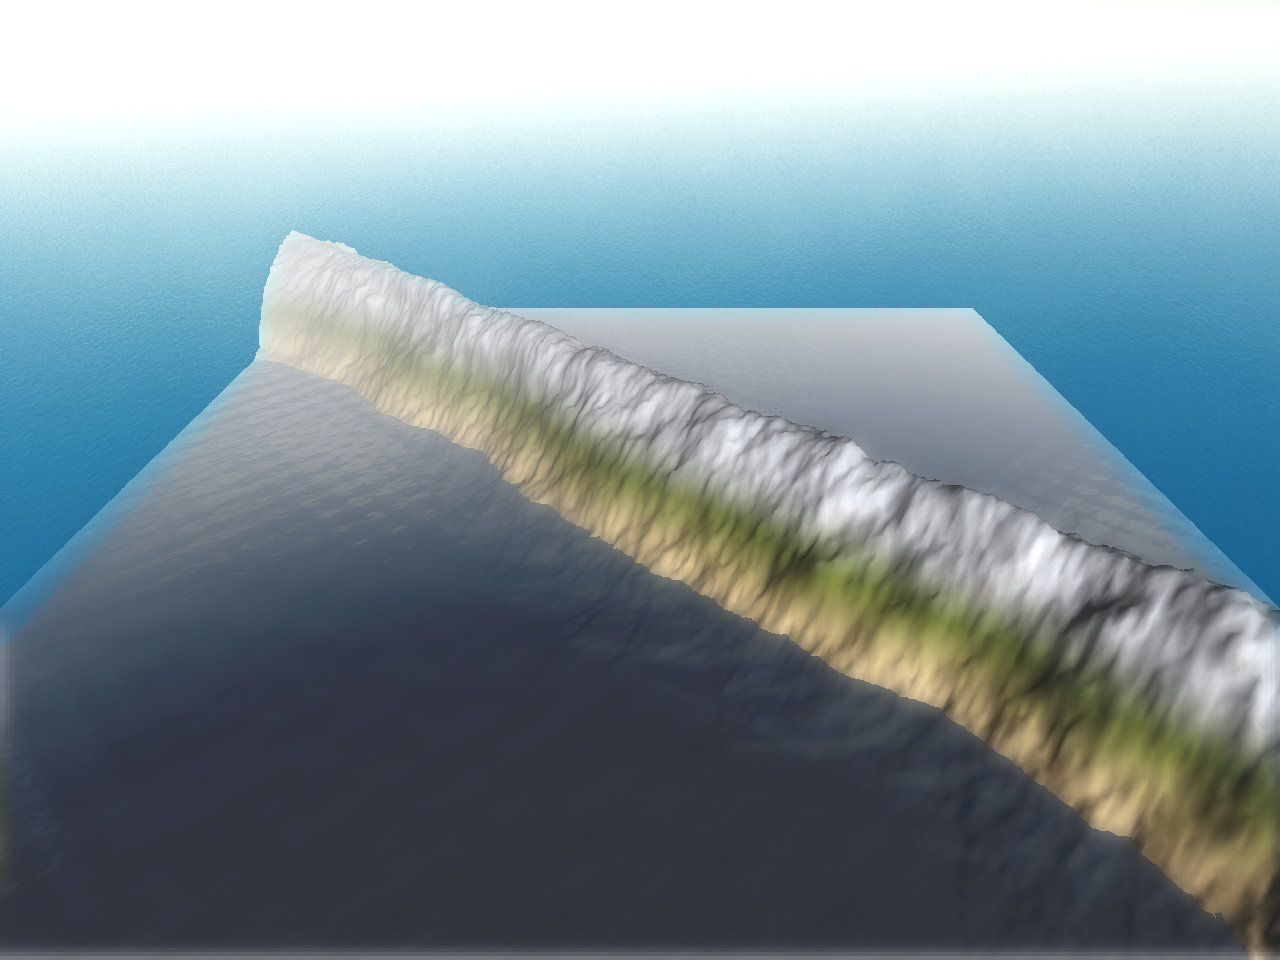
\includegraphics[width=\linewidth]{mountain-range-alteration.png}
  \caption{Each affected area raised by a random amount}\label{fig:mountainrangealteration}
\endminipage
\end{figure}

\section{Thermal erosion algorithm variations}
Fast terrain generation algorithms, like fault algorithm, produce very rough and spiky terrain features. Therefore terrain generated by fault algorithm has to be smoothed before usage. For this purpose thermal erosion algorithm can be used. It is capable of removing spikes and smoothing the terrain in general. Based on the roughness of the terrain, the following 2 variations of thermal erosion should be considered:
\begin{itemize}
  \item Height-aware thermal erosion
  \item Constant thermal erosion
\end{itemize}
In general, height-aware thermal erosion is a very good choice for almost any terrain roughness. It considers material hardness based on height which results in very realistic terrain transformations. However, experiments show that for very rough and spiky terrain, constant thermal erosion is preferable over height-aware thermal erosion since the latter causes heavy loss of detail in lower elevations and keeps spikes in higher elevations unaffected. These effects can be witnessed in \cref{fig:thermalbefore,fig:thermalafter1,fig:thermalafter2}.
\begin{figure}[!htb]
\minipage{0.33\textwidth}
  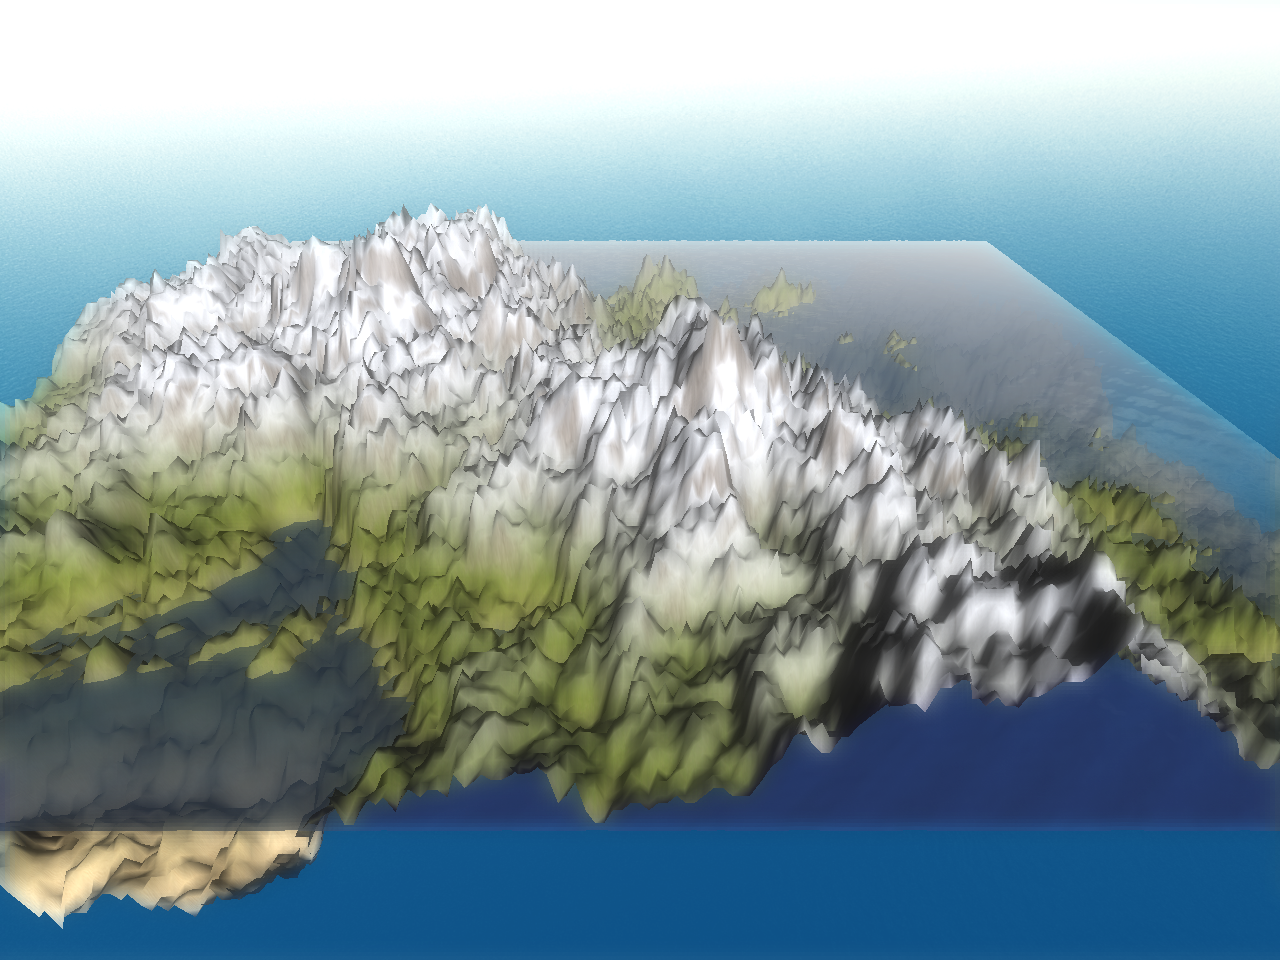
\includegraphics[width=\linewidth]{thermal-50-iterations-before.png}
  \caption{Heightmap generated with Fault algorithm}\label{fig:thermalbefore}
\endminipage\hfill
\minipage{0.33\textwidth}
  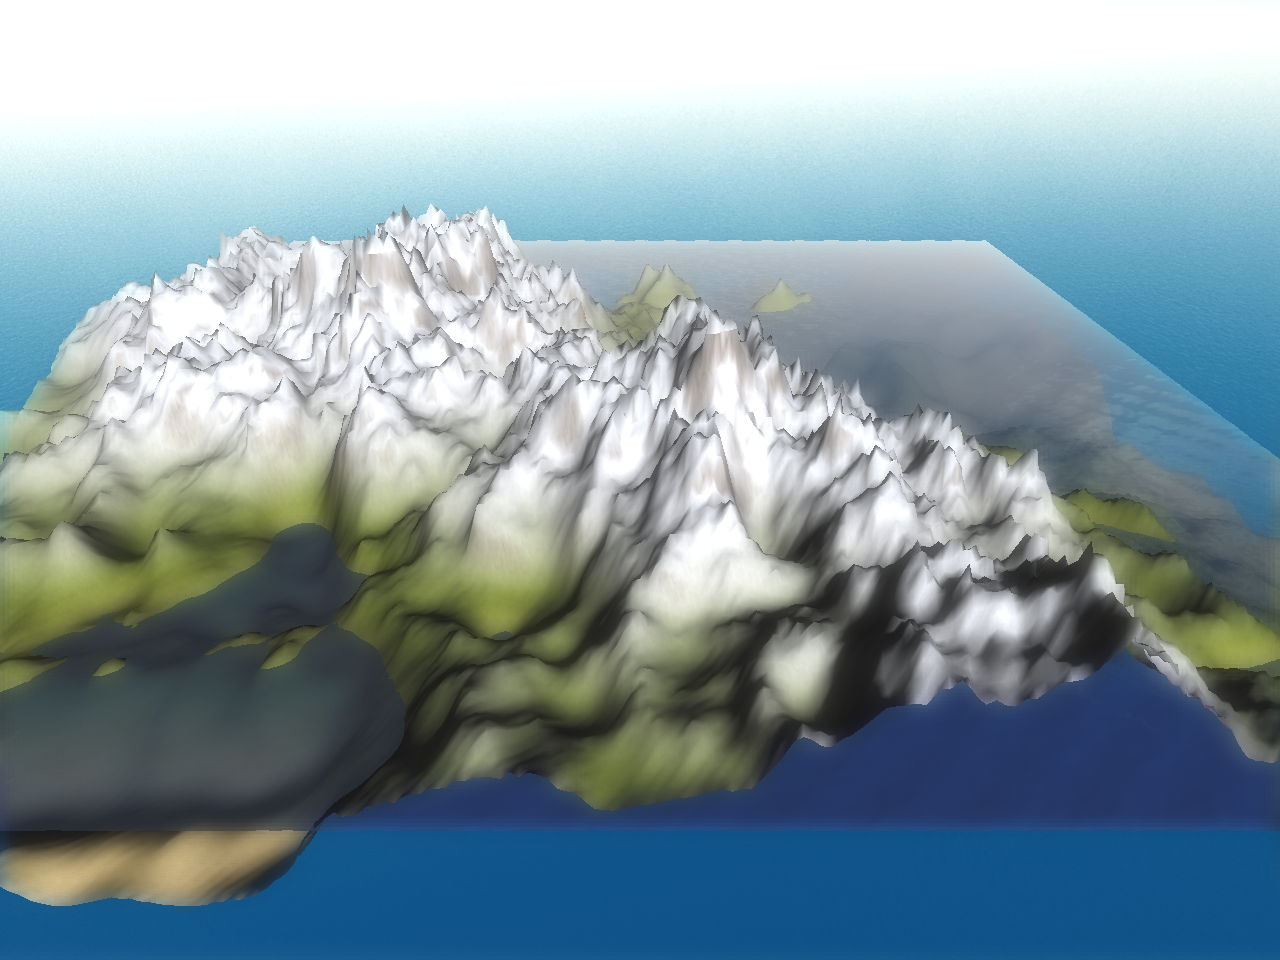
\includegraphics[width=\linewidth]{thermal-50-iterations-after1.png}
  \caption{Height-aware thermal erosion}\label{fig:thermalafter1}
\endminipage\hfill
\minipage{0.33\textwidth}%
  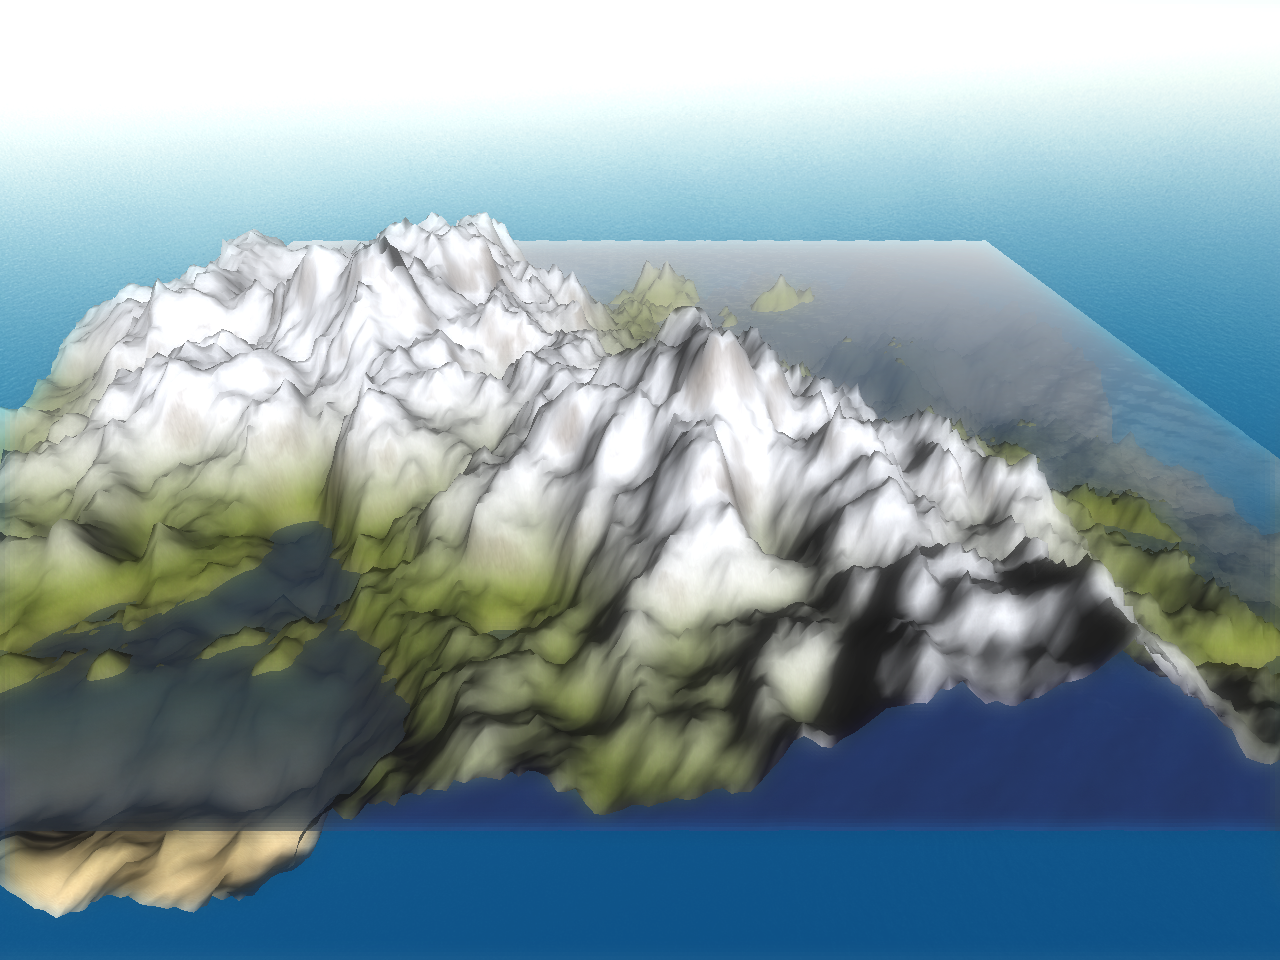
\includegraphics[width=\linewidth]{thermal-50-iterations-after2.png}
  \caption{Constant thermal erosion}\label{fig:thermalafter2}
\endminipage
\end{figure}

\section{Graph- and Voronoi-based RMP performance analysis}
The goal of this performance analysis is to compare two totally different implementations of RMP algorithm. The graph-based algorithm consists of several expensive steps including a minimal-cycle-search as well as a depth-first-search. These calculations solely take place on the CPU. The Voronoi-based algorithm takes full advantage of the GPU by generating Voronoi diagrams using the method described in \cref{subsec:voronoibasedimpl}. Both algorithms were given three tasks which required them to generate a single mountain of increasing complexity in the middle of a blank heightmap. The level of mountain complexity was determined by the amount of polygons generated in each iteration. The amount of polygons generated by the graph-based RMP algorithm is influenced by the number of cuts placed per iteration. Using Euler's formula also known as the \emph{Lazy Carterer's Sequence} \cite{Moore:1991} it is possible to calculate the maximum number of polygons $p$ generated by placing $n$ cuts per iteration:
\begin{align}
  p = \frac{n^2 + n + 2}{2}
\end{align}
The amount of polygons generated by the Voronoi-based RMP algorithm is directly influenced by the number of cones placed per iteration. Each task consisted of 100 iterations to ensure measurability. By repeating each task 10 times it was possible to reduce the noise to a neglectable amount. The experiment was performed on a MacBook Pro (2.8GHz Intel Core i5 processor, Intel Iris onboard graphics). \Cref{tab:graphperformanceanalysis,tab:voronoiperformanceanalysis} show the recorded results.
\begin{table}[h]
\centering
\caption{Graph-based RMP performance analysis}
\label{tab:graphperformanceanalysis}
\begin{tabular}{|r|r|r|r|}
\hline
 & Task 1 & Task 2 & Task 3 \\ \hline
\# of cuts & 3 & 4 & 5 \\ \hline
max. \# of polygons & 7 & 11 & 16 \\ \hline
\# of iterations & 100 & 100 & 100 \\ \hline
sample 1 & 2.93s & 45.47s & 5891.85s \\ \hline
sample 2 & 3.01s & 35.41s & 5921.50s \\ \hline
sample 3 & 2.80s & 43.66s & 5929.62s \\ \hline
sample 4 & 3.01s & 39.26s & 5962.49s \\ \hline
sample 5 & 3.02s & 59.81s & 5941.39s \\ \hline
sample 6 & 2.98s & 53.29s & 5957.13s \\ \hline
sample 7 & 3.05s & 48.87s & 5942.96s \\ \hline
sample 8 & 2.93s & 49.97s & 5965.95s \\ \hline
sample 9 & 3.02s & 49.33s & 5889.50s \\ \hline
sample 10 & 3.00s & 42.22s & 5971.09s \\ \hline
$\mu$ & 2.975s & 46.729s & 5937.348s \\ \hline
$\sigma^2$ & $5.27 \cdot 10^{-3}\textrm{s}$ & 50.139s & 855.362s \\ \hline
$\sigma$ & $7.26 \cdot 10^{-2}\textrm{s}$ & 7.081s & 29.247s \\ \hline
\end{tabular}
\end{table}
\begin{table}[h]
\centering
\caption{Voronoi-based RMP performance analysis}
\label{tab:voronoiperformanceanalysis}
\begin{tabular}{|r|r|r|r|}
\hline
 & Task 1 & Task 2 & Task 3 \\ \hline
\# of cones & 7 & 11 & 16 \\ \hline
\# of polygons & 7 & 11 & 16 \\ \hline
\# of iterations & 100 & 100 & 100 \\ \hline
sample 1 & 2.04s & 2.06s & 1.99s \\ \hline
sample 2 & 1.99s & 1.96s & 2.06s \\ \hline
sample 3 & 1.96s & 1.94s & 2.04s \\ \hline
sample 4 & 2.01s & 1.97s & 2.01s \\ \hline
sample 5 & 1.99s & 2.00s & 1.99s \\ \hline
sample 6 & 1.98s & 1.97s & 2.10s \\ \hline
sample 7 & 2.03s & 2.19s & 2.03s \\ \hline
sample 8 & 1.98s & 1.96s & 1.99s \\ \hline
sample 9 & 1.95s & 1.97s & 2.02s \\ \hline
sample 10 & 1.96s & 2.02s & 2.02s \\ \hline
$\mu$ & 1.989s & 2.004s & 2.025s \\ \hline
$\sigma^2$ & $8.99 \cdot 10^{-4}\textrm{s}$ & $5.49 \cdot 10^{-3}\textrm{s} $ & $1.23 \cdot 10^{-3}\textrm{s}$ \\ \hline
$\sigma$ & $3.00 \cdot 10^{-2}\textrm{s}$ & $7.41 \cdot 10^{-2}\textrm{s}$ & $3.5 \cdot 10^{-2}\textrm{s}$ \\ \hline
speedup & 1.496 & 23.318 & 2932.024 \\ \hline
\end{tabular}
\end{table}
The results clearly show the benefits of Voronoi-based RMP. Voronoi-based RMP algorithm scales much better than graph-based RMP algorithm. While graph-based RMP algorithm already slows down significantly generating 11 randomly distributed polygons, the Voronoi-based alternative seems to perform about the same regardless of the number of polygons to be generated. This behaviour is very valuable for realtime applications and therefore the Voronoi-based RMP algorithm was chosen over the graph-based alternative. With the graph-based RMP algorithm out of the picture, it would also be interesting to find the limits of the Voronoi-based alternative. For this reason another experiment was conducted. This time up to 100000 polygons were generated per iteration and the duration $t$ was noted down after each task consisting of 100 iterations was completed. \Cref{fig:voronoiperformancestresstest} shows a plot of the data recorded during this experiment.
\begin{figure}[h]
\centering
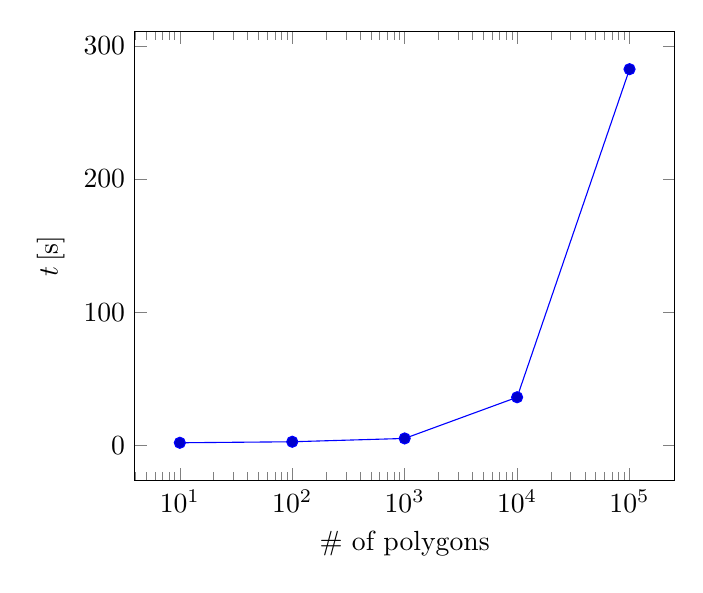
\begin{tikzpicture}
\begin{axis}[
    xlabel=\# of polygons,
    xmode=log,
    ylabel=$t\,\textrm{[s]}$,
]
\addplot table {
10 2.07
100 2.83
1000 5.32
10000 36.23
100000 282.46
};
\end{axis}
\end{tikzpicture}
\caption{Voronoi performance stress test}
\label{fig:voronoiperformancestresstest}
\end{figure}
The plot clearly shows that the Voronoi-based RMP algorithm is capable to generate up to 1000 polygons per iteration in realtime. For realtime terrain generation, fast generation of huge amounts of randomly distributed polygons is a huge deal. Not only is it possible to control the spread of a mountain with high precision, it is also possible to generate more detailed mountains in general.

%----------------------------------------------------------------------------------------
\chapter{Conclusion \& Future Work}
\label{sec:concl}

Lorem ipsum dolor sit amet, consetetur sadipscing elitr, sed diam nonumy
eirmod tempor invidunt ut labore et dolore magna aliquyam erat, sed diam voluptua. At
vero eos et accusam et justo duo dolores et ea rebum. Stet clita kasd gubergren, no sea
takimata sanctus est Lorem ipsum dolor sit amet. Lorem ipsum dolor sit amet, consetetur
sadipscing elitr, sed diam nonumy eirmod tempor invidunt ut labore et dolore magna
aliquyam erat, sed diam voluptua. At vero eos et accusam et justo duo dolores et ea
rebum. Stet clita kasd gubergren, no sea takimata sanctus est Lorem ipsum dolor sit amet.



%----------------------------------------------------------------------------------------
% Bibliography
%----------------------------------------------------------------------------------------

\bibliographystyle{plain}
\bibliography{literature}

\end{document}
